\pagebreak
\chapter{VBA}
\setcounter{section}{0}
\section{Das VBA-Tutorial}
\subsection{Grundlagen}
\subsubsection{Debug.Print}
Diese Funktion $Debug$ in \gls{VBA} ist ein Objekt, welches zwei Methoden besitzt. Diese sind $Print$ und $Assert$. Die $Print$ Methode erlaubt das einfache Wiedergeben der Werte von Variablen in \gls{VBA}. Der Vorteil gegenüber $MsgBox$ ist, dass ein keine Bestätigung der Ausgabe erfolgen muss. Ebenso bleibt die Darstellung im Direktfenster nach Beendigung der Prozedur erhalten.
\begin{figure}[H]
	\centering
	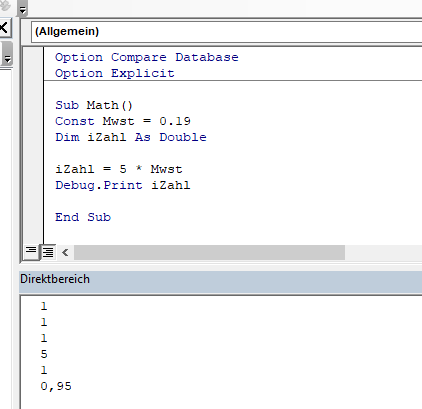
\includegraphics[scale = 0.3]{attachment/chapter_2/Scc026}
	\caption{}
	\label{fig:Scc026}
\end{figure} 
\subsubsection{Array}
Ein Array in \gls{VBA} wird über $()$ indiziert. Dabei kann ein Array jeglichen Datentypen enthalten.
\begin{lstlisting}[style=VBA]
Option Compare Database
Option Explicit

Sub Math()

	Dim sAusgabe(2) As String
	
	sAusgabe(0) = "Test im Feld 0"
	Debug.Print sAusgabe(0) ' Test im Feld 0
	
	sAusgabe(1) = "Test im Feld 1" 'Test im Feld 1
	Debug.Print sAusgabe(1)
	
End Sub
\end{lstlisting} 
Die Dimensionalisierung des Arrays kann auch über ein Variable erfolgt. Ebenso kann das Array auch neu definiert werden. Dafür wird $ReDim$ verwendet.
Dim iAnzahl As Integer
\begin{lstlisting}[style=VBA]
Sub Math()

	iAnzahl = 3
	ReDim sFeld(iAnzahl)
	sFeld(0) = "Feld 0"
	Debug.Print sFeld(0) ' Feld 0
	
	iAnzahl = 4
	ReDim sFeld(iAnzahl)
	Debug.Print sFeld(0) ' Leer

End Sub
\end{lstlisting} 
\subsection{Objekte}
\subsubsection{Klassen}
Wie auch in der \gls{OOP} können über \gls{VBA} Klassen erstellt werden. Dabei wird das \textit{Klassen-Module} verwendet. Der Name des Klassenmoduls im \textit{Klassenmodule} Ordner ist das Objekt.
\begin{figure}[H]
	\centering
	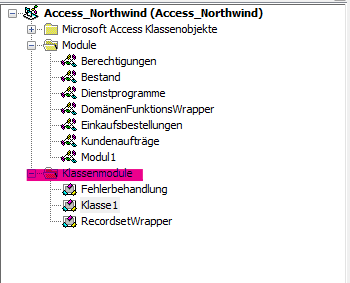
\includegraphics[scale = 0.3]{attachment/chapter_2/Scc027}
	\caption{}
	\label{fig:Scc027}
\end{figure} 
Am Beispiel des \textit{Autos} wird die Klasse \textbf{Auto} geschaffen. Die Klasse ist zwar leer, aber in \gls{VBA} wird sie schon als Klasse erkannt. Dies kann nachvollzogen werden, wenn in einem \textit{Standardmodul} eine Variable vom Typ der Klasse Auto erzeugt wird.
\begin{figure}[H]
	\centering
	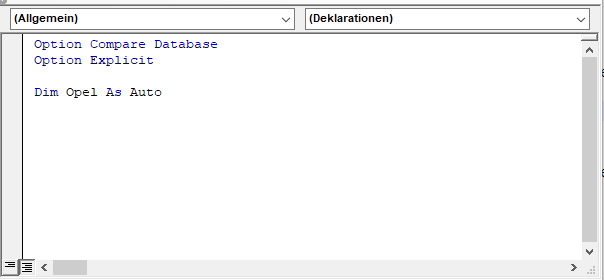
\includegraphics[scale = 0.6]{attachment/chapter_2/Scc028}
	\caption{}
	\label{fig:Scc028}
\end{figure} 
Das Symbole
\begin{figure}[H]
	\centering
	
\includegraphics[scale = 1.3]{attachment/chapter_2/Scc029}
	\caption{}
	\label{fig:Scc029}
\end{figure} 
zeigt dabei Auto als Objekt an. \textcolor{red}{Wichtig:} Die Dimensionierung einer Objektvariablen ist nur ein \textit{Verweis}. Die Erzeugung des Objekte wird durch 
\begin{align}
	\textcolor{blue}{Set }\dots = \textcolor{blue}{ New} \text{ Auto}
\end{align}
instanziiert. Sollen mehrere Auto erzeugt werden, so lässt sich dies durch weitere Objektverweise erzeugen.
\begin{lstlisting}[style=VBA]
Dim Opel As Auto
Dim VW As Auto
Dim Ferrari As Auto
\end{lstlisting}
Wie schon erwähnt, sind die Objekte noch nicht instanziiert. Es folgt:
\begin{lstlisting}[style=VBA]
'Objektverweise
Dim Opel As Auto
Dim VW As Auto
Dim Ferrari As Auto

'Instanzisierung
Set Opel = New Auto
Set VW = New Auto
Set Ferrari As Auto
\end{lstlisting}
Der Vorgang kann ebenso auch in einer Zeile erfolgen.

\begin{lstlisting}[style=VBA]
Dim Opel As New Auto
\end{lstlisting}
Man spricht auch hier von \textit{Objektdeklaration}. 
\subsubsection{Methoden}
Methoden werden in \gls{VBA} mit dem Symbole
\begin{figure}[H]
	\centering
	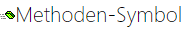
\includegraphics[scale = 1.3]{attachment/chapter_2/Scc030}
	\caption{}
	\label{fig:Scc030}
\end{figure} 
dargestellt. \\

Für die Klasse \textit{Auto} wird die Methode \textit{hupen} definiert. Diese ist der Klasse zu gewissen und kann über die Klasse abgerufen werden. Eine Methode wird mit eine Prozedur definiert. 
\begin{figure}[H]
	\centering
	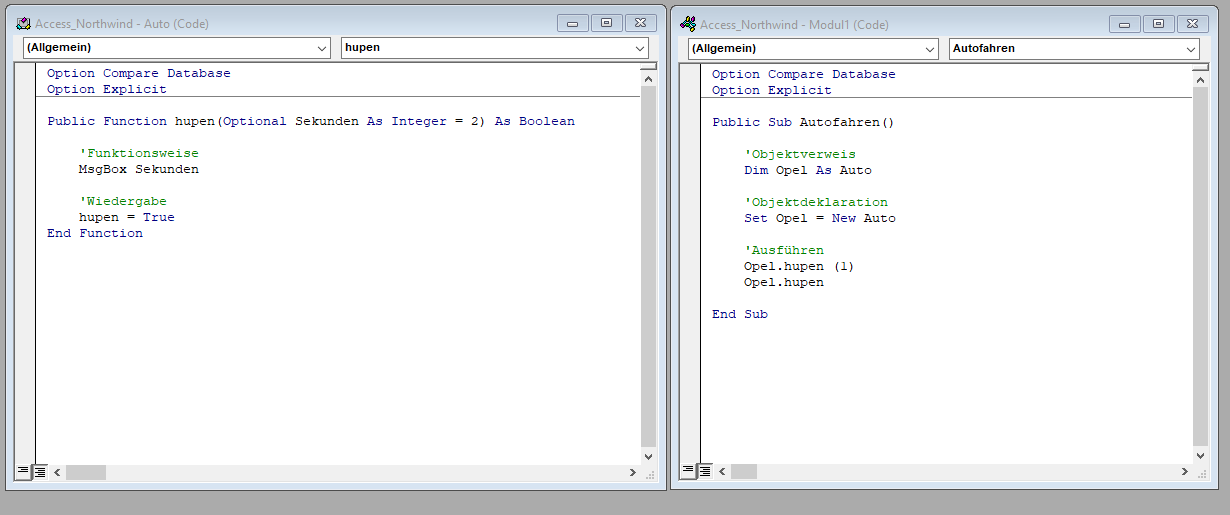
\includegraphics[scale = 0.3]{attachment/chapter_2/Scc031}
	\caption{}
	\label{fig:Scc031}
\end{figure} 
Die Funktion (Mehtode) $hupen()$ verwendet eine Optionale Variable. Dabei wird mit $=2$ der voreingestellt Wert definiert, welcher verwendet wird, wenn die kein Wert übergeben wird. Oder kurzgesagt: \textit{Default}.
Die Syntax wie Variablen eingegeben werden, kann mit $()$ oder ohne erfolgen.
\subsubsection{Eigenschaft}
\paragraph{Property} 
Zusätzlich zu den Methoden einer Klasse, können auch Eigenschaften definiert werden. Im einfachsten Fall sind dies Intrinsische Variablen. Es können aber auch weitere Objekte als Eigenschaft definiert werden.\\ 
Eigenschaften werden in mit \gls{g_IS} mit dem Symbole:
\begin{figure}[H]
	\centering
	
\includegraphics[scale = 0.7]{attachment/chapter_2/Scc032}
	\caption{}
	\label{fig:Scc032}
\end{figure} 
dargestellt. Damit werden einzelnen Variablen, Unterobjekte und Property Prozeduren angesprochen. \\
Wird das Objekt \bl{Opel} der Klasse \bl{Auto} über ein Modul initalisiert, so stehen alle Eigenschaften und Methoden.  
\begin{figure}[H]
	\centering
	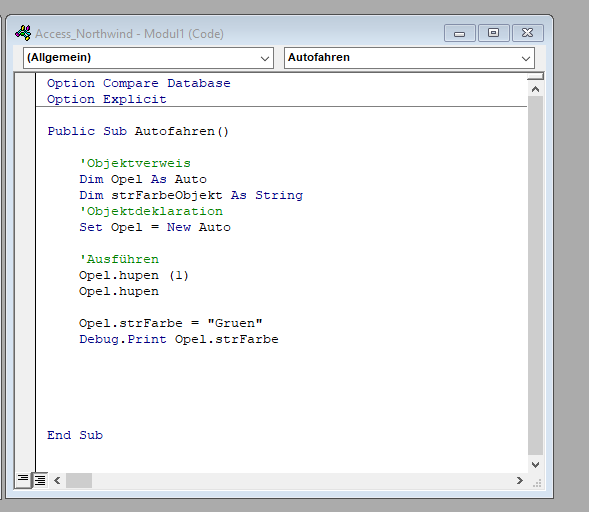
\includegraphics[scale = 0.3]{attachment/chapter_2/Scc037}
	\caption{}
	\label{fig:Scc037}
\end{figure}
\paragraph{Property Prozedur}
Die Eigenschaften zu einer Klasse können \textcolor{blue}{public} oder \textcolor{blue}{privat} sein. Wenn sie öffentlich hinterlegt sind, können diese über den Klassenverweis direkt geändert werden. Variablen die \textcolor{blue}{private} sind, können nur über die Klasse selber geändert werden.\\
Die \textcolor{blue}{Property Let}/ \bl{Get} Prozedure hilft die Eingabe von Daten für die Eigenschaften zu verwalten. Dies bittet sich vorwiegend für Variablen vom Typ \bl{private} an. Eine mögliche Variante die Verwaltung zu steueren, ist die privaten Variablen mit dem Prefix $pv$ zu versehen. Die Prozedur hingegen, kann den Variablennamen tragen ohne Prefix. Gleichnamigkeit der Variable und der dazugehörigen Prozedur ist nicht vorgesehen. Es ist aber möglich, das \bl{Get} und \bl{Let} den gleichen Namen tragen.   
Wie schon erwähnt, werden die Prozeduren als Eigenschaften geführt und nicht als Methoden angezeigt.
\begin{itemize}
	\item Verwendet man nur \bl{Property Let}, so ist eine Konfiguration der Variable vorgesehen, aber ein Auslesen nicht.
	\item \bl{Property Set} erlaubt eine Adressierung von Referenzen von Objekten.
	\item Verwendet man nur \bl{Property Get}, so ist eine \bl{private} Variable schreibgeschützt. 
\end{itemize}
Am Beispiel des Objektes \textit{Opel} werden die Eigenschaften über die \bl{Property} Prozedur verwaltet. Bei \bl{Get} wird auch der Rückgabewert definiert. Dabei verhält sich \bl{Get} wie eine Funktion und \bl{Let} wie ein \bl{Sub}.
\begin{figure}[H]
	\centering
	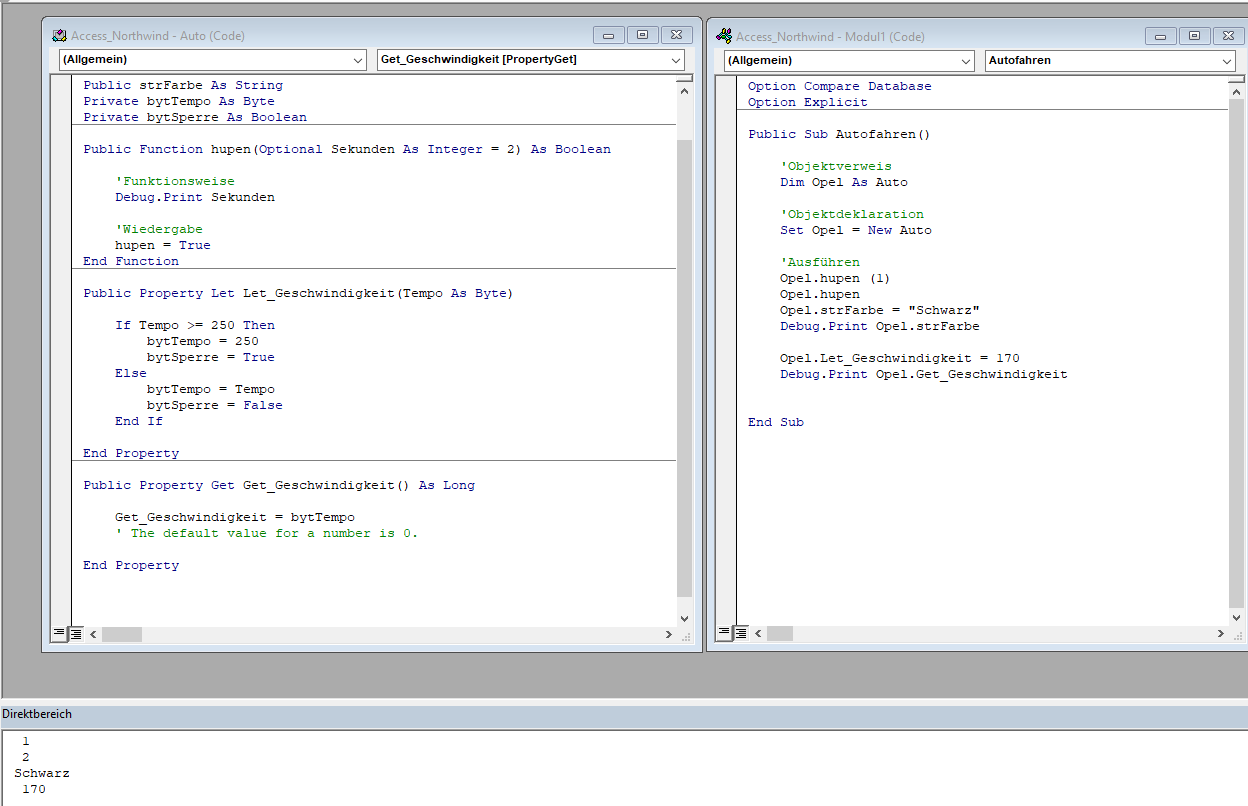
\includegraphics[scale = 0.3]{attachment/chapter_2/Scc033}
	\caption{}
	\label{fig:Scc033}
\end{figure} 

Für die Deklaration von Eigenschaften wird meist die \bl{Property} Prozedur verwendet. Eine Deklaration außerhalb einer Prozedur ist nicht in VBA vorgesehen.
\begin{figure}[H]
	\centering
	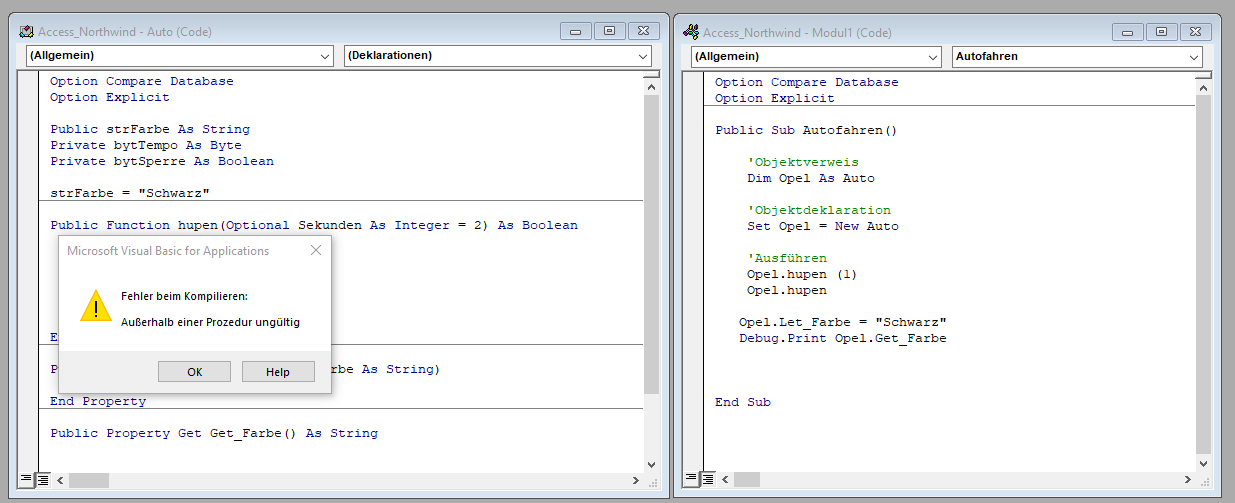
\includegraphics[scale = 0.3]{attachment/chapter_2/Scc034}
	\caption{Keine Deklaration der Variablen außerhalb einer Prozedur}
	\label{fig:Scc034}
\end{figure} 
Innerhalb der Methoden kann dies jedoch vorgenommen werden.
\begin{figure}[H]
	\centering
	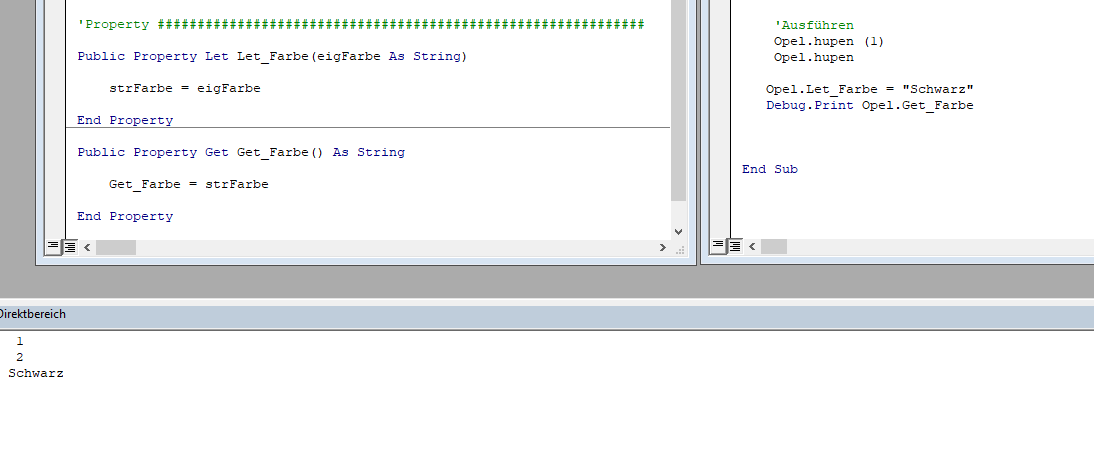
\includegraphics[scale = 0.3]{attachment/chapter_2/Scc035}
	\caption{Deklaration der Variablen mit Hilfe von \bl{Property}}
	\label{fig:Scc035}
\end{figure} 
Erfolgt die Deklaration in dem \textit{Modul}, so ist nichts weiter zu tun. 
Der große Vorteil bei der \bl{Property} Prozedur ist, dass für \bl{Let} und \bl{Get} der gleiche Name verwendet werden kann. 
Es kann somit eine \bl{private} Variable definiert werden, und diese über eine \bl{Get} und \bl{Let} abgerufen und verändert werden. 

\begin{figure}[H]
	\centering
	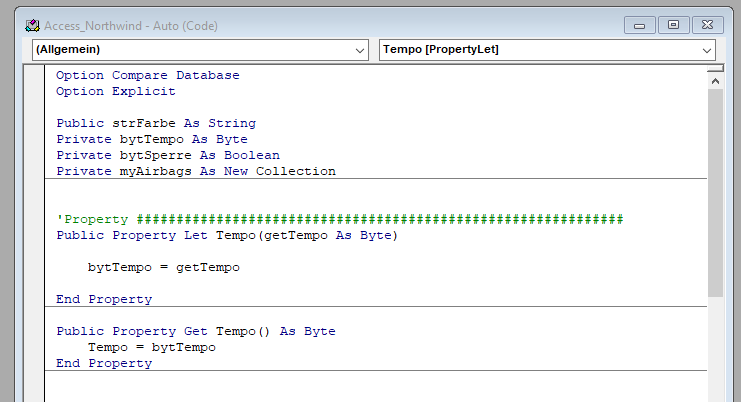
\includegraphics[scale = 0.3]{attachment/chapter_2/Scc040}
	\caption{}
	\label{fig:Scc040}
\end{figure}

\paragraph{Unterobjekte}
Das Ziel soll sein, das ein Objekt ebenfalls aus mehreren Unterobjekten bestehen kann. Dafür werden Eigenschaften verwandt, welche als Objektevariablen definiert werden. \\

Die Klasse Radio wird mit einer Eigenschaft und einer Methode gefüllt.
\begin{figure}[H]
	\centering
	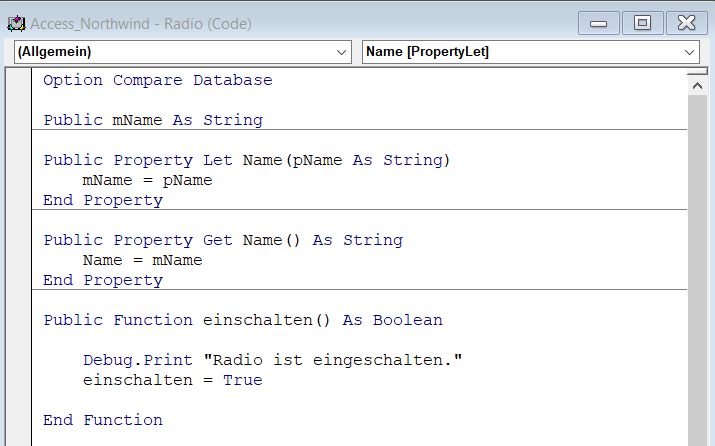
\includegraphics[scale = 0.3]{attachment/chapter_2/Scc038}
	\caption{}
	\label{fig:Scc038}
\end{figure} 
In der Klasse Auto wird die Eigenschaft $ppRadio$ vom Typ \bl{Radio} deklariert. Damit zu jedem Objekt ein Radio initalisert wird, wird die $Class_Initialize$ Prozedur aufgerufen. Diese wird immer angestoßen, wenn ein neues Objekt initializiert wird.  
\begin{figure}[H]
	\centering
	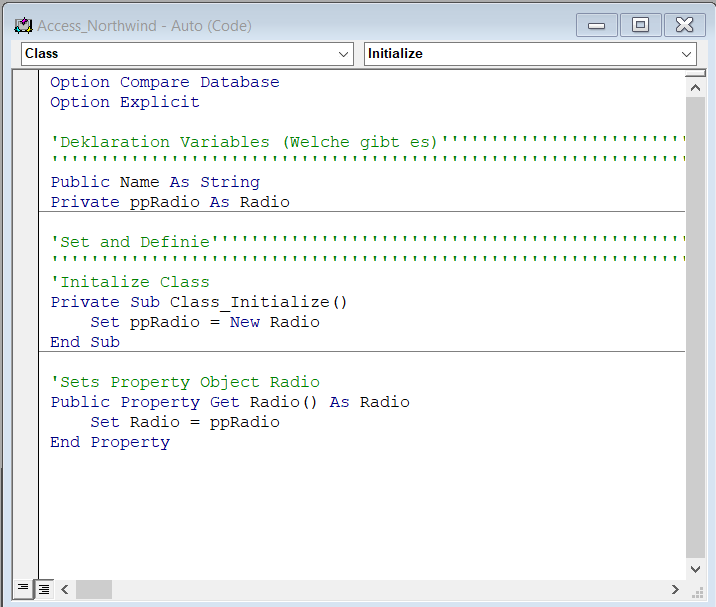
\includegraphics[scale = 0.3]{attachment/chapter_2/Scc039}
	\caption{}
	\label{fig:Scc039}
\end{figure} 
Mit dem Ausdruck $Set ppRadio = New Radio$ wird das Unterobjekt initializiert. Die Get-Prozedur gibt den Verweis wieder. Dabei ist die Get-Prozedur vom Typ Radio. Mit $Set Radio = ppRadio$ wird der Verweis an die Funktion übergeben. Hier müsste nochmal geprüft werden, ob Set benötigt wird.\\
Am Ende kann das Radio mit seinen Eigenschaften und Methden zu jedem initalizierten Auto abgerufen werden.
\begin{figure}[H]
	\centering
	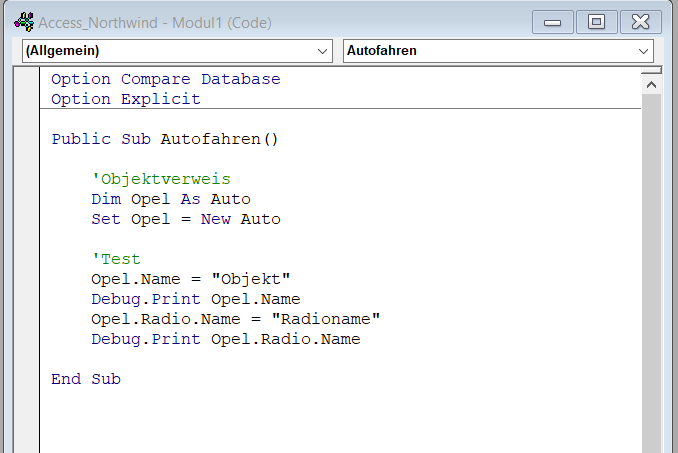
\includegraphics[scale = 0.3]{attachment/chapter_2/Scc041}
	\caption{}
	\label{fig:Scc041}
\end{figure} 
\subsubsection{Auflistung}
Eine \textbf{Auflistung} ist ein Objekt, welches vor definierte Methoden hat:
\begin{itemize}
	\item Item - Diese erlaubt eine Zugriff auf die Elemente in \textit{Collection} Objekt.
	\item Count - Zählt wie viele Elemente eine Auflistung besitzt.
	\item Add - Fügt ein Element der Auflistung hinzu.
	\item Remove - Entfernt ein Element aus der Auflistung.
	\item \begin{figure}[H]
		\centering
		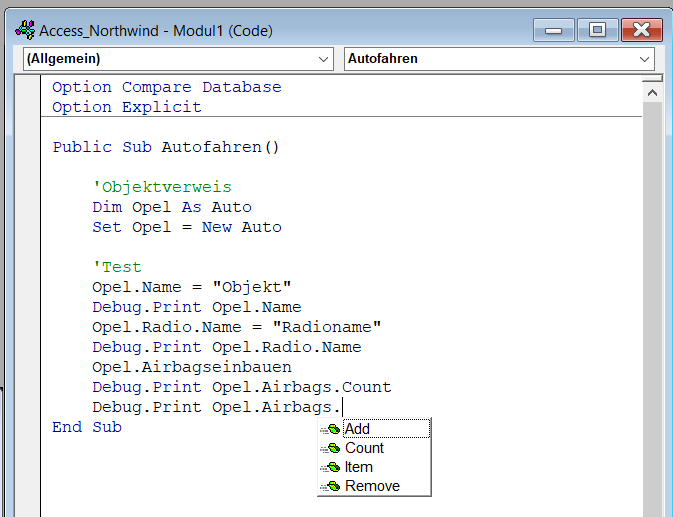
\includegraphics[scale = 0.3]{attachment/chapter_2/Scc042}
		\caption{}
		\label{fig:Scc042}
	\end{figure}
\end{itemize}

An Hand des Auto-Beispiels muss Auflistung deklariert:
\begin{figure}[H]
	\centering
	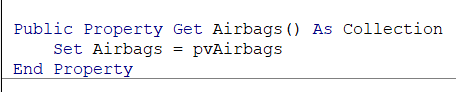
\includegraphics[scale = 0.3]{attachment/chapter_2/Scc044}
	\caption{}
	\label{fig:Scc044}
\end{figure} 
und initaliziert
\begin{figure}[H]
	\centering
	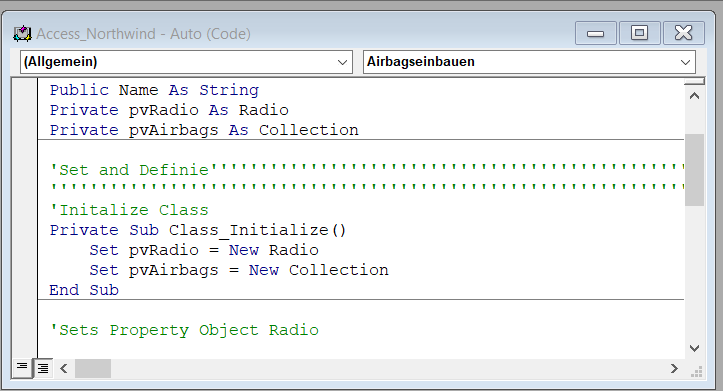
\includegraphics[scale = 0.3]{attachment/chapter_2/Scc045}
	\caption{}
	\label{fig:Scc045}
\end{figure} 
werden. In dem genannten Beispiel sollen zwei Airbags eingebaut werden. Dafür greift die Klasse Auto auf die Klasse Airbag zu und speichert diese im Objekt Airbags.
\begin{figure}[H]
	\centering
	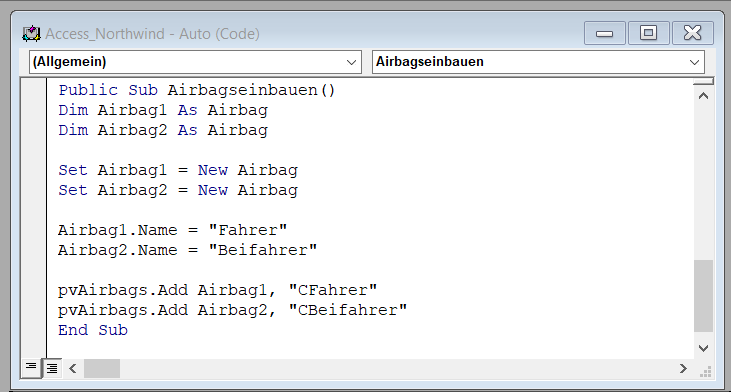
\includegraphics[scale = 0.3]{attachment/chapter_2/Scc043}
	\caption{}
	\label{fig:Scc043}
\end{figure}
Über das Modul kann die Auflistung angesteuert werden, dafür gibt es verschiedene Syntaxen für eine Aufrufung der einzelne Elemente.
\begin{figure}[H]
	\centering
	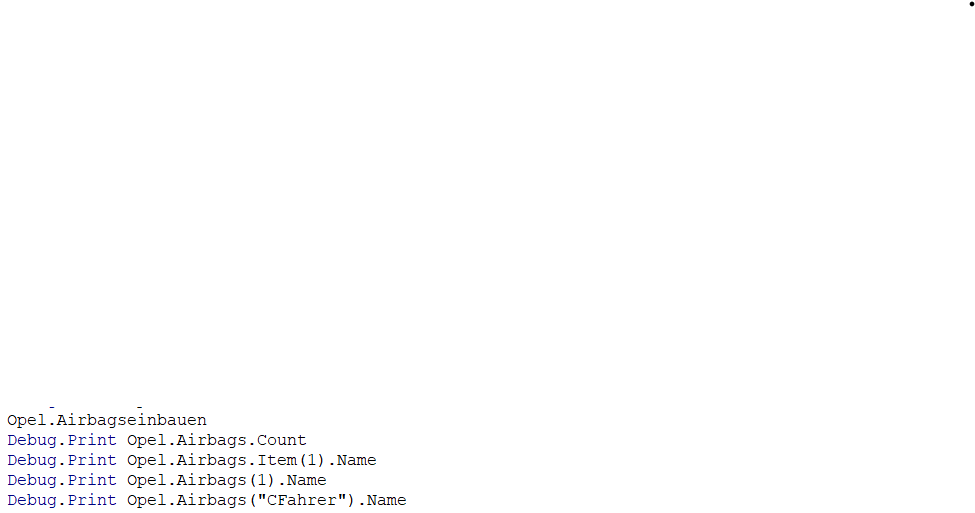
\includegraphics[scale = 0.3]{attachment/chapter_2/Scc046}
	\caption{}
	\label{fig:Scc046}
\end{figure}
\subsubsection{Ereignisse}
Ereignisse sind Prozeduren, welche nicht über das Objekt selbst abgerufen werden können, sondern durch Vorgänge mit dem Objekt hervorgerufen werden.
Zwei Prozeduren haben wir schon kennengelernt. Für \textbf{Ereignisse} wird das Symbole
\begin{figure}[H]
	\centering
	
\includegraphics[scale = 0.3]{attachment/chapter_2/Scc052}
	\caption{}
	\label{fig:Scc052}
\end{figure}
verwendet. Im Objektkatalog wird diese neben Eigenschaften und Methoden angezeigt.
\begin{figure}[H]
	\centering
	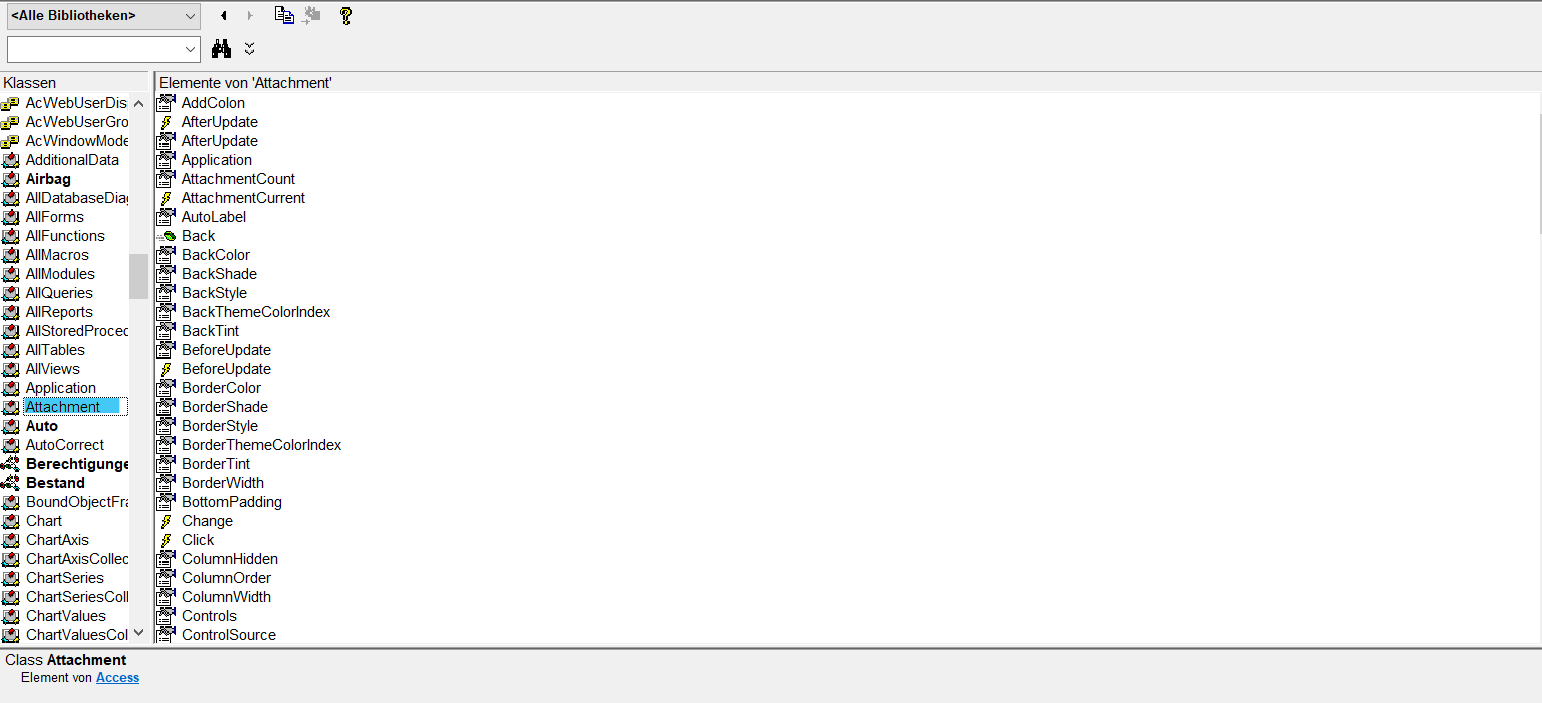
\includegraphics[scale = 0.3]{attachment/chapter_2/Scc051}
	\caption{}
	\label{fig:Scc051}
\end{figure}
Unter einem VBA-Application Objekt findet auf der linken Seite des Drop-Down
\subsubsection{Objektanweisung}
Zwei Anweisungen, \bl{With... End With} und \bl{For Each}, sind für das Referenzen von Objekten wichtig.
Es kann ein spezifisches Objekt angesteuert mit der With-Umgebung:
\begin{lstlisting}[style=VBA]
With Objekt 
.Methode
.Eigenschaft
.Objekt.Methode
End With
\end{lstlisting}
Als Beispiel
\begin{lstlisting}[style=VBA]
Private Sub AddCustomer()
Dim theCustomer As New Customer

With theCustomer
.Name = "Coho Vineyard"
.URL = "http://www.cohovineyard.com/"
.City = "Redmond"
End With

With theCustomer.Comments
.Add("First comment.")
.Add("Second comment.")
End With
End Sub

Public Class Customer
Public Property Name As String
Public Property City As String
Public Property URL As String

Public Property Comments As New List(Of String)
End Class
\end{lstlisting}
Mit dem \bl{For Each} Loop können die verschiedenen Elemente in einer Auflistung angesteuert werden.
\begin{lstlisting}{style=VBA}
	For Each Element-Objekt in Auflistung
		'Statement
	Next
\end{lstlisting}
Dies geschieht solange bis alle Objekt in der Auflistung durchlaufen sind.
Anhand des Beispiels zum Airbageinbau können muss ein Airbag Objekt zu erst seperat deklariert werden.
\begin{lstlisting}[style=VBA]
	Public Sub Autofahren()
	
	'Objektverweis
	Dim Opel As Auto
	Set Opel = New Auto
	Dim LAirbag As Airbag
	
	
	'Test
	Opel.Name = "Objekt"
	Debug.Print Opel.Name
	Opel.Radio.Name = "Radioname"
	Debug.Print Opel.Radio.Name
	Opel.Airbagseinbauen
	Debug.Print Opel.Airbags.Count
	Debug.Print Opel.Airbags.Item(1).Name
	Debug.Print Opel.Airbags(1).Name
	Debug.Print Opel.Airbags("CFahrer").Name
	Debug.Print Opel.Airbags.Item(2).Name
	Debug.Print Opel.Airbags.Item(2).einbauen
	For Each LAirbag In Opel.Airbags
	Debug.Print LAirbag.Name 'Fahrer, Beifahrer
	Next
	End Sub
\end{lstlisting}

\subsubsection{Me-Object}
Wenn Makros geschrieben werden, kann dies in zwei Formen getan werden:
\begin{itemize}
	\item Modules
	\item Class-Modules
	\begin{itemize}
		\item Mit einem Interface
		\item Ohne Interface
	\end{itemize}
\end{itemize}
Es gibt also Klassen-Module, welche ein Interface-Desgin mit sich bringen.
Das $ME$-Objekt hilft, die Adressierung in einem Module zu verallgemeinern. In Excel werden Tabellenbläter als \textit{Excel-Klassenobjekte} in \gls{VBA}. Am Beispiel von Northwind wird gezeigt:

\begin{figure}[H]
	\centering
	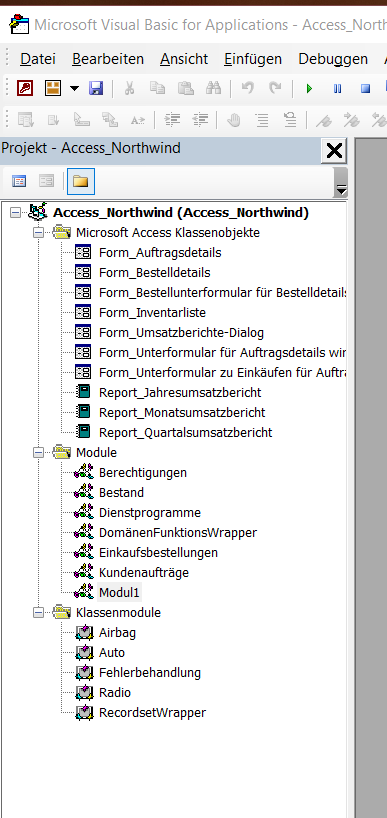
\includegraphics[scale = 0.3]{attachment/chapter_2/Scc053}
	\caption{}
	\label{fig:Scc053}
\end{figure} 
Access weißt Form und Reports als Klassenobjekte aus. Die weiteren Module wurden ergänzt und die Klassenmodul sind die Objekte, welcher selber gewählt wurden.
Wird ein Marco geschrieben, welches sich in einem Klassenmodule befindet, so kann das Objekt direkt mit $ME.$ angesteuert werden. \\
Am Beispiel von Excel wird ein Wert $"$Hello Friends$"$ der Zelle $"$A1$"$ des Datenblattes $"$Dat Sheet$"$ gespeichert. 
\begin{figure}[H]
	\centering
	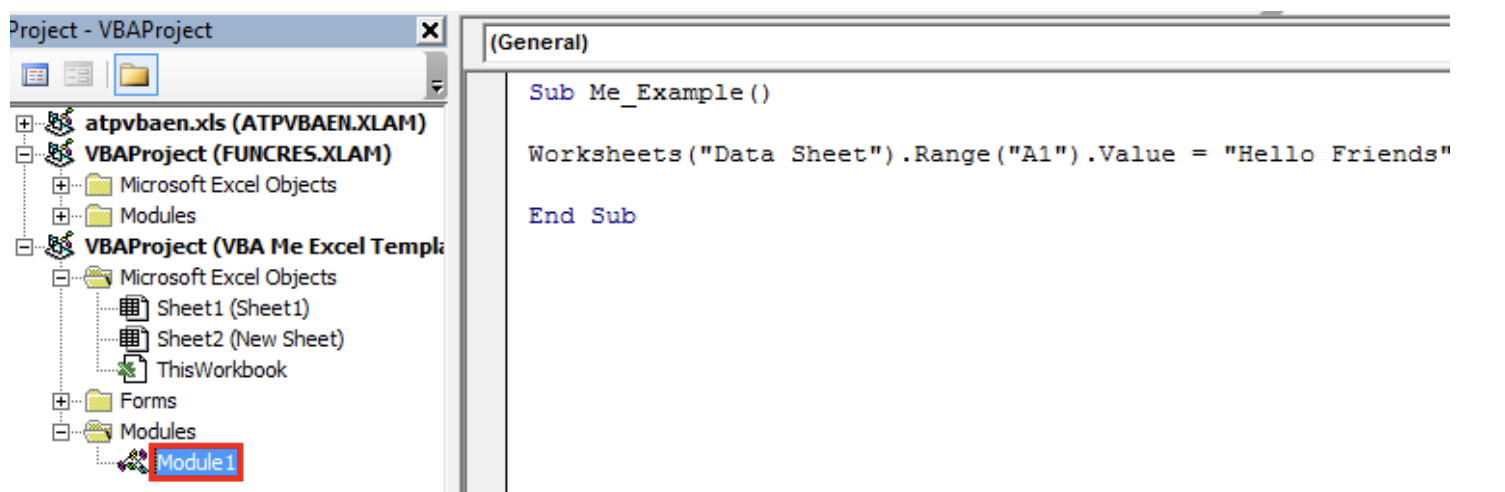
\includegraphics[scale = 0.3]{attachment/chapter_2/Scc054}
	\caption{}
	\label{fig:Scc054}
\end{figure}
Dieser Code könnte jedoch auch im Microsoft Excel Objekt \textit{Sheet2 (Data Sheet)} (Achtung: Im Bild steht $"$New Sheet$"$) eingetragen werden. Die Adressierung des Objekte mit
\begin{lstlisting}[style=VBA]
Worksheet("Data Sheet").
\end{lstlisting}
könnte auch über 
\begin{lstlisting}[style=VBA]
Me.
\end{lstlisting}
erfolgen. \gls{g_IS} erkennt dies ebenfalls, und weißt die zugehörigen Methoden und Ereignisse aus.
\begin{figure}[H]
	\centering
	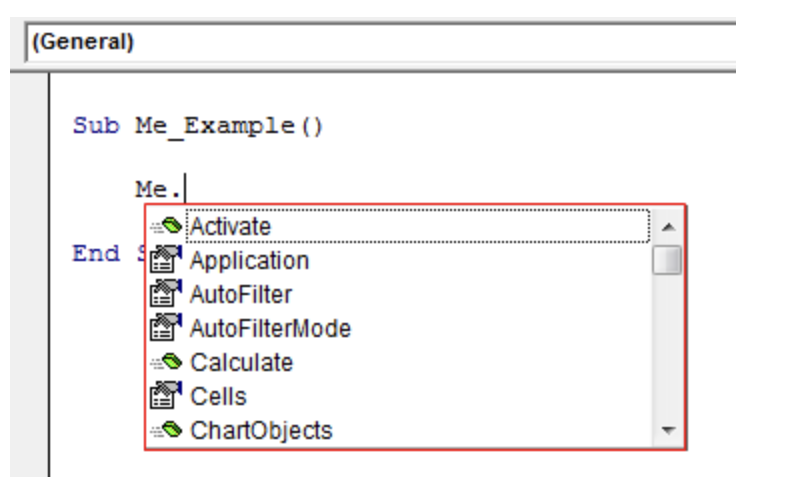
\includegraphics[scale = 0.3]{attachment/chapter_2/Scc055}
	\caption{}
	\label{fig:Scc055}
\end{figure}
Das Sub im Klassenobjekt selbst sieht dann wie folgt aus:
\begin{lstlisting}[style=VBA]
Sub Me()
Me.Range("A1").Value = "Hello Friends"
End Sub
\end{lstlisting}
Der Vorteil der sich daraus ergibt, ist, dass der Code leichter wiederverwendet werden kann. 
Gleiches gilt für \textit{Userforms}. Ein Userform ist ein intanziertes Objekt. Objekt-Eigenschaften können erzeugt werden und haben eine visuelles Erscheinungsbild. Die Ansteuerung kann in einem Userform-Module ebenfalls über $ME.$ erfolgen.
\begin{figure}[H]
	\centering
	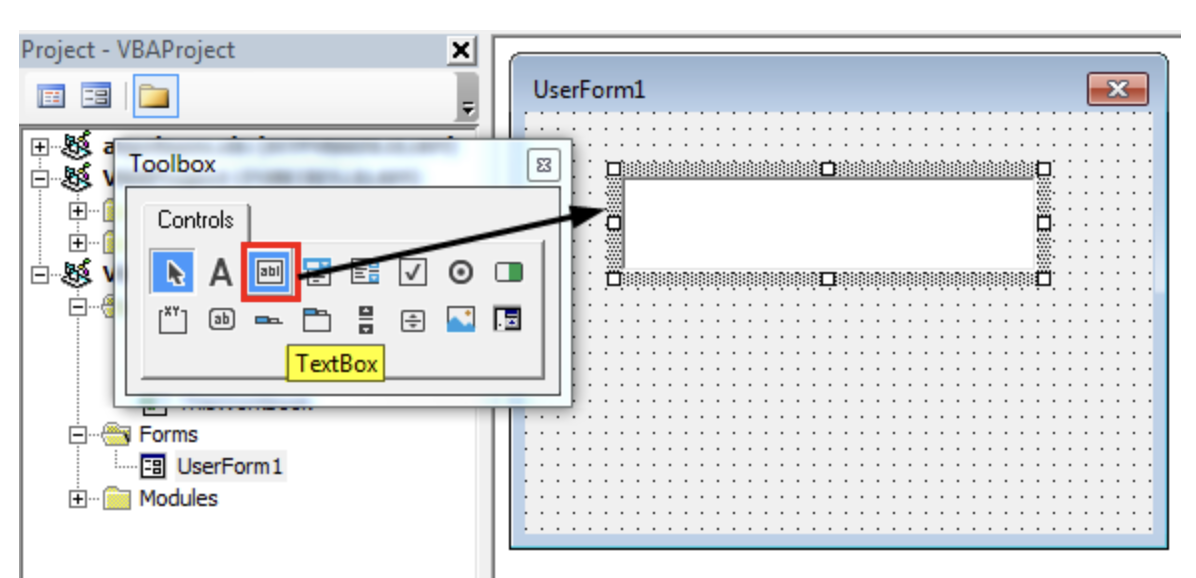
\includegraphics[scale = 0.3]{attachment/chapter_2/Scc056}
	\caption{}
	\label{fig:Scc056}
\end{figure}
\begin{lstlisting}[style=VBA]
Private Sub TextBox_Change()
	UserForm1.TextBox1.Text = "Welcome to VBA!"
End Sub
\end{lstlisting}
oder 
\begin{lstlisting}[style=VBA]
Private Sub TextBox_Change()
	ME.TextBox1.Text = "Welcome to VBA!"
End Sub
\end{lstlisting}
mit dem Ergebnis
\begin{figure}[H]
	\centering
	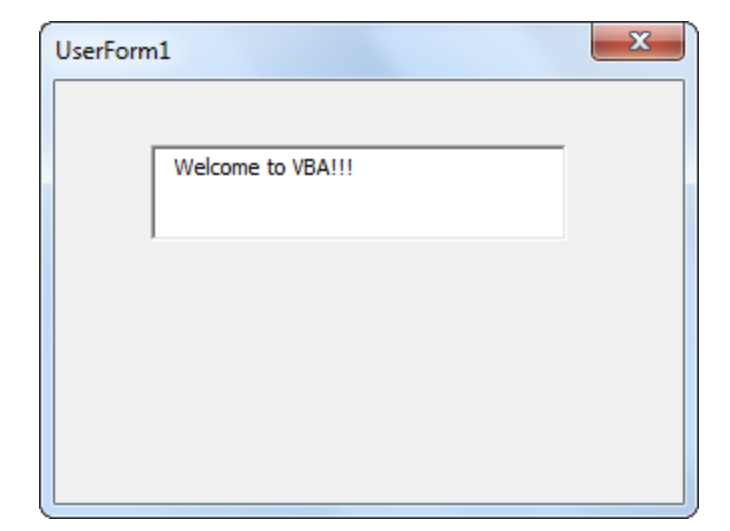
\includegraphics[scale = 0.3]{attachment/chapter_2/Scc057}
	\caption{}
	\label{fig:Scc057}
\end{figure}
\subsubsection{Objektmodell}
Bei der Programmierung eigener Objekt, ist es innvoller die Objektstruktur zu dokumentieren. Im Fall von Northwind würde diese wie folgt aussehen:
\begin{figure}[H]
	\centering
	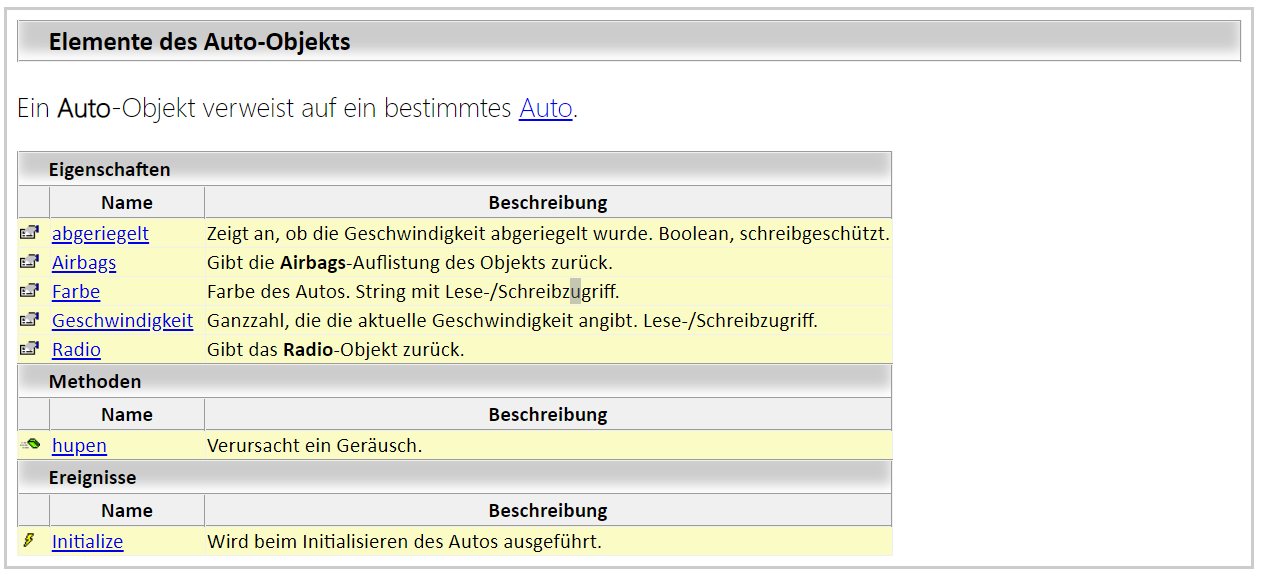
\includegraphics[scale = 0.3]{attachment/chapter_2/Scc058}
	\caption{}
	\label{fig:Scc058}
\end{figure}

\subsection{Fehlerbehandlung}
\begin{description}
	\item[Error Resume Next] Fehler in der Zeile werden ignoriert. Die Prozedur wird daraufhin so ausgeführt, als wäre die Zeile nicht existent.
	\item[On Error go to] Tritt ein Fehler auf, wir auf an einen definierten Punkt im Code gesprungen. Hier muss aufgepasst werden, dass die Übersichtlichkeit gewahrt wird, und die Funktion sollte nur zur Fehlerbehebung verwendet werden. Der Verweis kann ein Wort oder Zahl gefolgt von einem $:$.
\begin{lstlisting}[style=VBA]
Function GibFehler() As Double
Dim i As Double

On Error GoTo Eingabefehler

i = 1 / InputBox("Geben Sie eine Zahl ein")

GibFehler = i

Exit Function

Eingabefehler:
GibFehler = 0

End Function
\end{lstlisting}
	\item[Resume] Mit Resume kann wider zurück in den Code gesprungen werden. Zum Beispiel wird eine Schleife, basierend an dem Fehler weiter durchlaufen. Vermerk: \bl{Err} Objekt fängt den Fehler einer Zeile ab. Mit \bl{Err.Number} kann der Fehlerwert wiedergegeben werden. 
\begin{lstlisting}[style=VBA]

Function GibFehler()
Dim i As Byte

On Error GoTo Eingabefehler

i = InputBox("Geben Sie eine Zahl ein")
i = (i ^ 2 + 1) / i

GibFehler = i

Ende:
Exit Function

Eingabefehler:
Select Case Err.Number
    Case 6  'Überlauf (negativer Wert)
        Resume
    Case 11 'Division durch "0"
        i = 0
        Resume Next
    Case 13 'Typen unverträglich (Text)
        Resume Ende
End Select

End Function
\end{lstlisting}
\end{description}
\subsection{Kurzer Einblick Formular}
\begin{description}
\item[Combbox] Zufügen der Werte für eine Combbox.
\begin{lstlisting}[style=VBA]
Privat Sub UserForm1_Initialize()
Dim Liste(2) as Variant

Liste(0) = "A"
Liste(1) = "B"
Liste(2) = "C"

Me.ComboBox1.List = Liste
Me.ComboBox1.AddItem ("D")

End Sub
\end{lstlisting}
\end{description}
\subsection{Microsoft Access}
\subsubsection{Marcos, Module}
Access bietet die Möglichkeit \bl{Marcoaktionen} über ein Click-und-Drop-Modus zu generieren. Die Funktionen sind jedoch im Vergleich zu \bl{Modulen} starr. Alle Makroaktionen sind in \gls{VBA} über das \bl{DoCmd} Objekt abrufbar.
\subsubsection{Formulare, Reports}
\begin{itemize}
\item Formulare werden über das das Auflistungen \bl{Forms} angesteuert. Die Steuerelemente zugehörig zu einer Form werden über \bl{Control} verwaltet (Collection). 
\begin{lstlisting}[style=VBA]
Debug.Print Application.Forms(0).Control("txtName").Name
\end{lstlisting} 
\item \textbf{Ereignise} Die Steuerungselement eines Formulares können auf viele der Ereignisse reagieren.
\end{itemize} 
Am Beispiel von Nordwind enthält das \textit{Formular Inventarliste} viele Steuerelemente. 
\begin{figure}[H]
	\centering
	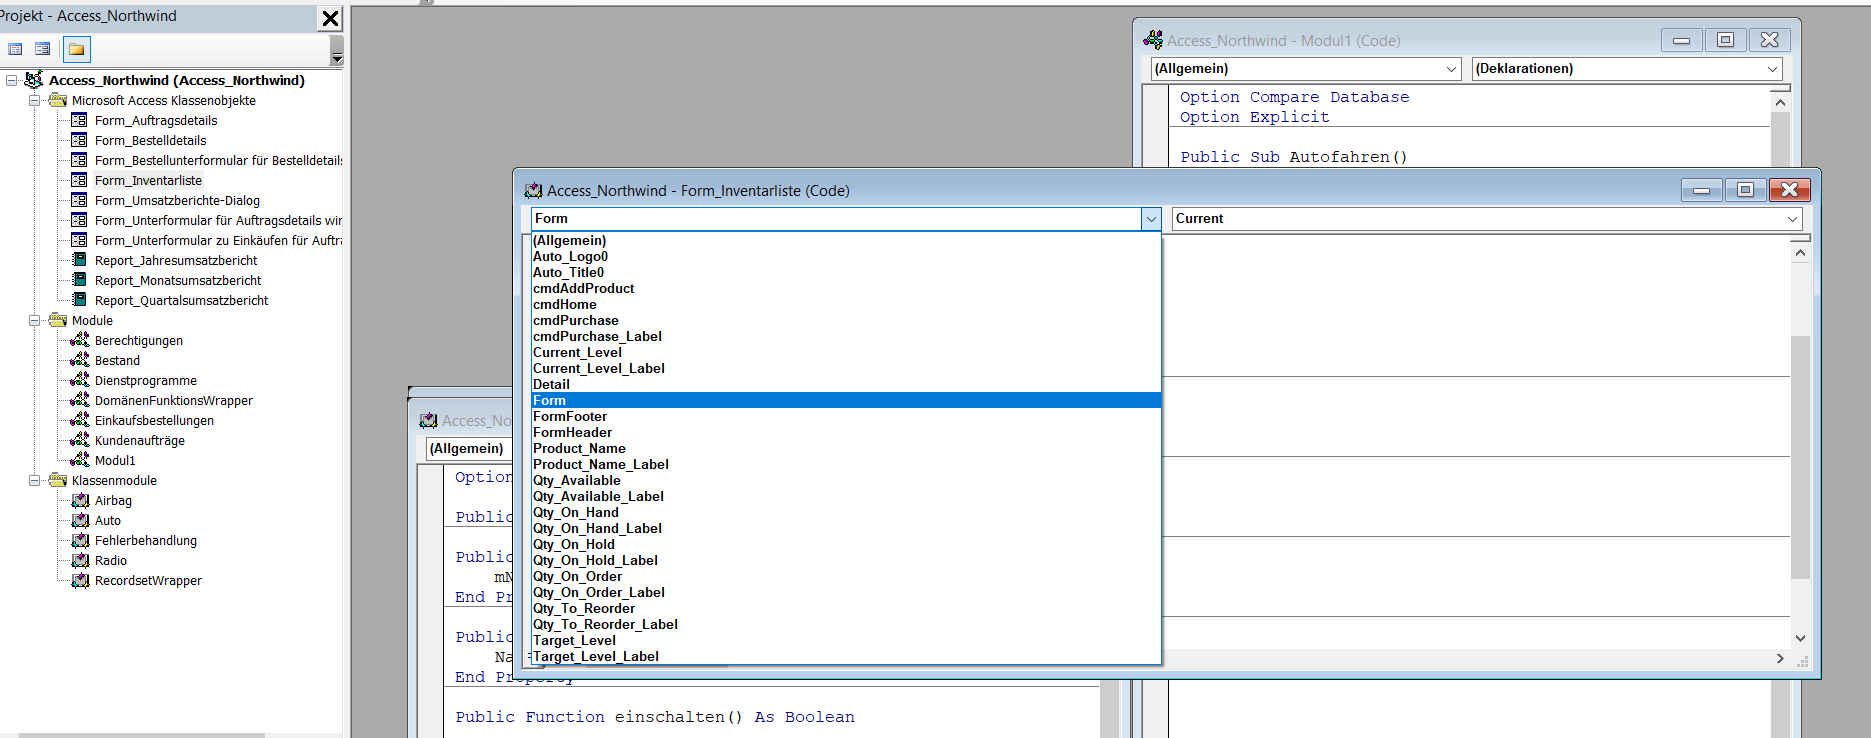
\includegraphics[scale = 0.3]{attachment/chapter_2/Scc059}
	\caption{}
	\label{fig:Scc060}
\end{figure}
Jedes dieser Element kann auf eine Vielzahl von \bl{Ereignissen}. 
\begin{figure}[H]
	\centering
	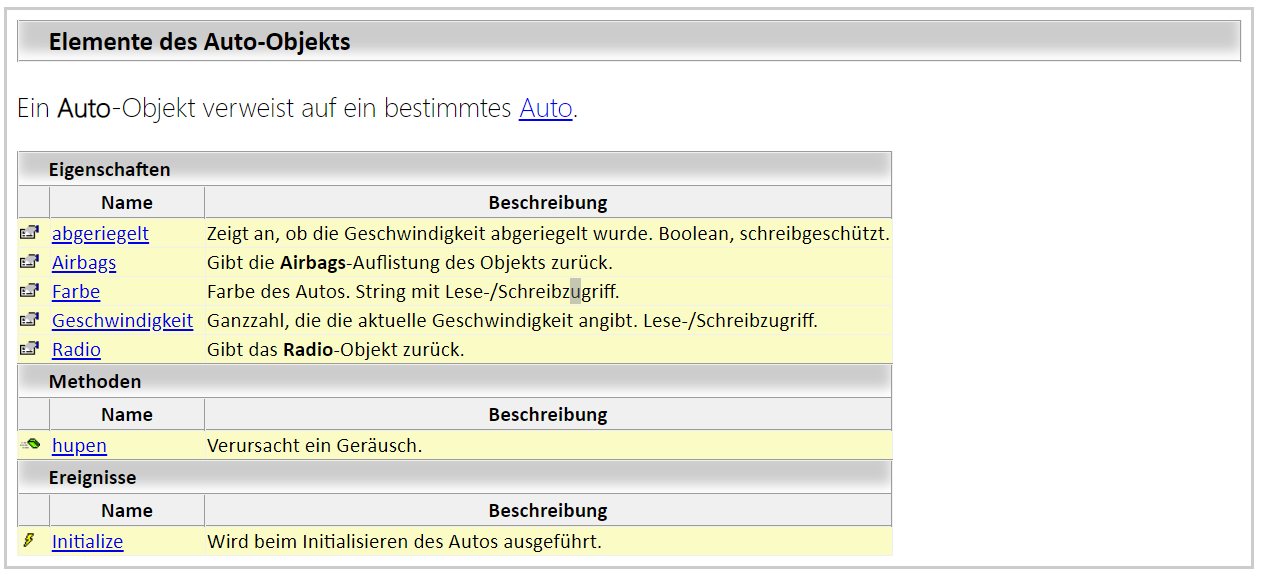
\includegraphics[scale = 0.3]{attachment/chapter_2/Scc058}
	\caption{}
	\label{fig:Scc060}
\end{figure}
\begin{lstlisting}[style=VBA]

Option Compare Database
Option Explicit

Private Sub Form_Current()
Me.txtNachname.BackColor = RGB(255, 128, 128)
End Sub

Private Sub txtNachname_AfterUpdate()
Me.txtNachname.BackColor = RGB(128, 128, 255)
End Sub

\end{lstlisting} 
\subsubsection{Tabellen}
\begin{itemize}
\item Der Zugriff auf Daten wird von Access nicht unterstützt. Dies geschieht alles über Datenbank Objekt Bibliotheken. Dabei ist die wichtigste für den einfachen Gebrauch \bl{DAO} (Database Object).
\item Für die Datenbasis in der eigenen Access-Datenbank wird gilt: DAO.Database = Currentdb
\item Um ein spezifischen Datentabelle zuladen wird DAO.Recordset = Currentdb.OpenRecordset("Name")
\end{itemize}  


\pagebreak
\section{VBA: Access}

\subsection{Sammelsurium}
\begin{itemize}
\item Close Recordset am Ende einer Prozedur: Recordset.Close Set Recordset to nothing
\item Close Database am Ende einer Prozedur, Set Variable to nothing
\item \textit{Recordset}.Move(Rows, [Optional]Bookmark): Rows ist ein Long-Parameter der notwendig ist. 
\item \item \textit{Recordset}.MoveNext() Bewegt sich 
\item \textit{Recordset}.AddNew(): Fügt eine neue Zeile zum Datenset und macht die zugefügte Zeile zum \textit{Current Record}. 
\item EOF: End of File gibt solange das Ende nicht erreicht ist den Wert \bl{false} wieder. 
\item Idee: Ein Form anlegen, welcher über die verschiedensten Forms und Reports ansteuert. Ebenso, sollten die Butten so angelegt werden, dass die man zurückspringen kann (Me-Objekt). Plus: Es sollten die anderen offenen Tabs geschloßen werden. 
\item DbEngine - DAO Objekt ist das übergeordneste Objekte. Es gibt auch keine Möglichkeit mehrere Instanzen davon zu erzeugen. Es existieren zwei große \bl{Auflistungen}: Workspaces und Errors.
\item Idee: Start-Seite: Hier werden alle wichtigen Informationen und Verlinkungen angezeigt.
\item Über die Eigenschaften der Aktuellen Datenbank kann der Name, sowie weitere Eigenschaften angepasst werden.
\begin{figure}[H]
	\centering
	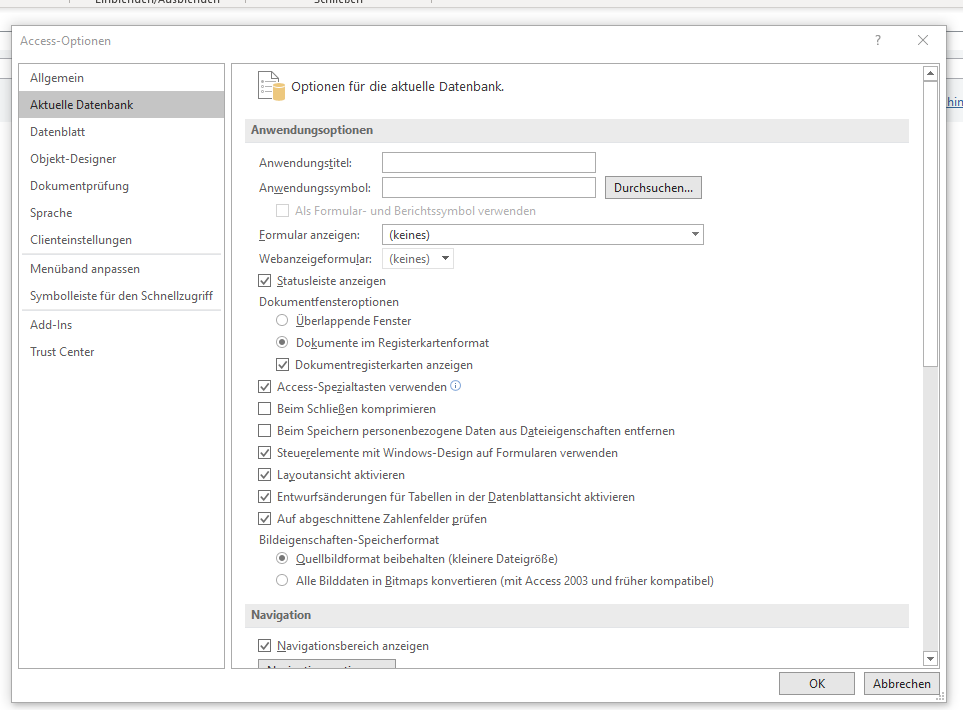
\includegraphics[scale = 0.3]{attachment/chapter_2/Scc064}
	\caption{}
	\label{fig:Scc064}
\end{figure}
\end{itemize}  

\subsection{Introduction VBA Basic}
\subsubsection{VBA Syntax}
\begin{description}
	\item[Method] siehe \gls{OOP}. Diese ist eine spezifische Funktion. Diese ist nur anwendbar für ein vorgegebenes Object oder einer Familie von vererbten Objekten. 
	\item[Function] A function is a piece of code that is called by name. It can be passed data to operate on (i.e. the parameters) and can optionally return data (the return value). All data that is passed to a function is explicitly passed.
	\item[Statment] Die ist ein einzeiliger Ausdruck. Dieser drück meist eine Aktion oder eine Definition aus.
	\begin{lstlisting}[style=VBA]
	Dim obj As Object ' one statment
	' ...
	If x = true then x = 1 else 5 ' one statment
	\end{lstlisting}
	Um mehrere Aktionen miteinander zu verbinden, wir $:$ verwendet.
	\begin{lstlisting}[style=VBA]
	'...
	rsDataSet.Close:          Set rsDataSet= Nothing
	'...
	\end{lstlisting}
	Mit der $With$ Funktion kann man mehrer statments zusammenfassen. Dabei ist es egal, das das statement aus mehreren Methoden abrufen besteht. 
	\begin{lstlisting}[style=VBA]
	'...
	With Currentdb.Sheet("Tabelle1").Range("B1")
	.Color = blue
	.Value = "This is a message."
	.Foreground = Brushes.DarkSeaGreen
	.Background = Brushes.LightYellow
	End With
	'...
	\end{lstlisting}
	Soll das statement unterbrochen werden, so verwendet man $\_$.
\end{description} 

\subsubsection{Object Modell for Access}  
Über die Seite zur Dokumentation für die Datenobjekte für \gls{VBA} im Office Context bietet eine umfassende Sammlung aller Objekte die im Access Kontext wichtig sind. 

\begin{figure}[H]
	\centering
	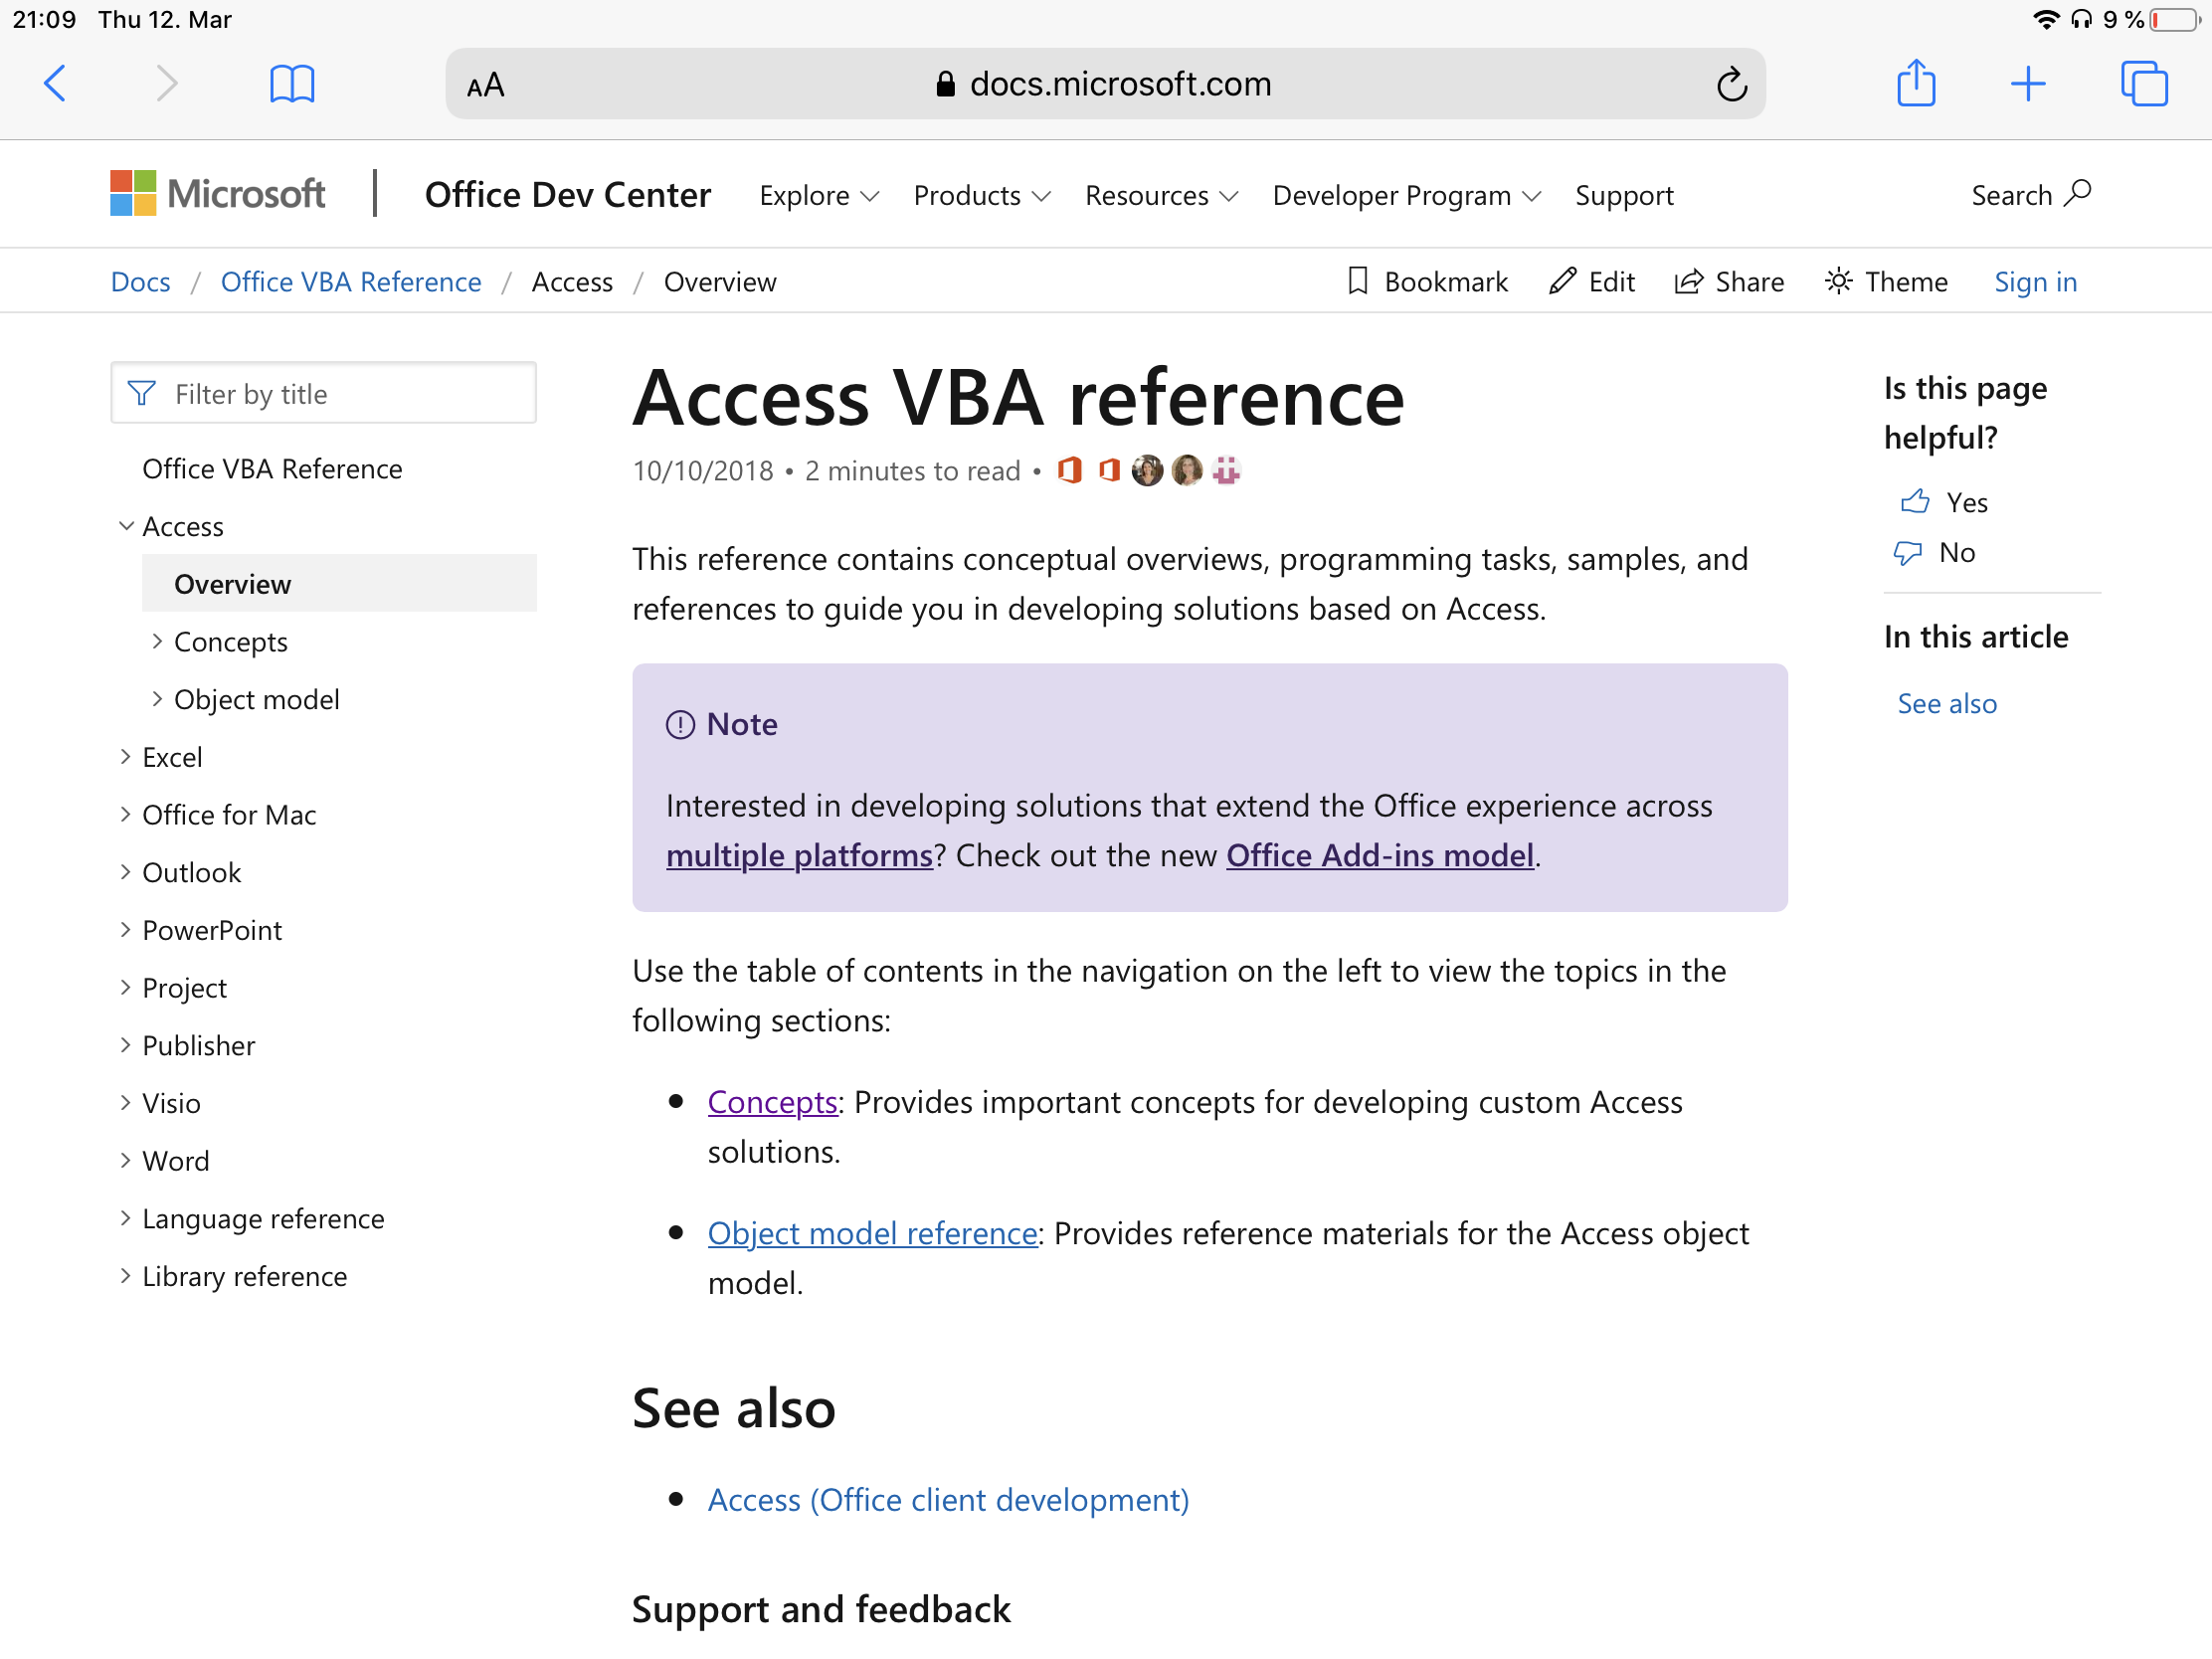
\includegraphics[scale = 0.3]{attachment/chapter_2/Scc019}
	\caption{}
	\label{fig:Scc019}
\end{figure} 
Es wird zwischen \textit{Concepts} und \textit{Objects} unterschieden. Im folgenden wird sich überwiegend auf Objekte fokussiert.


\begin{figure}[H]
	\centering
	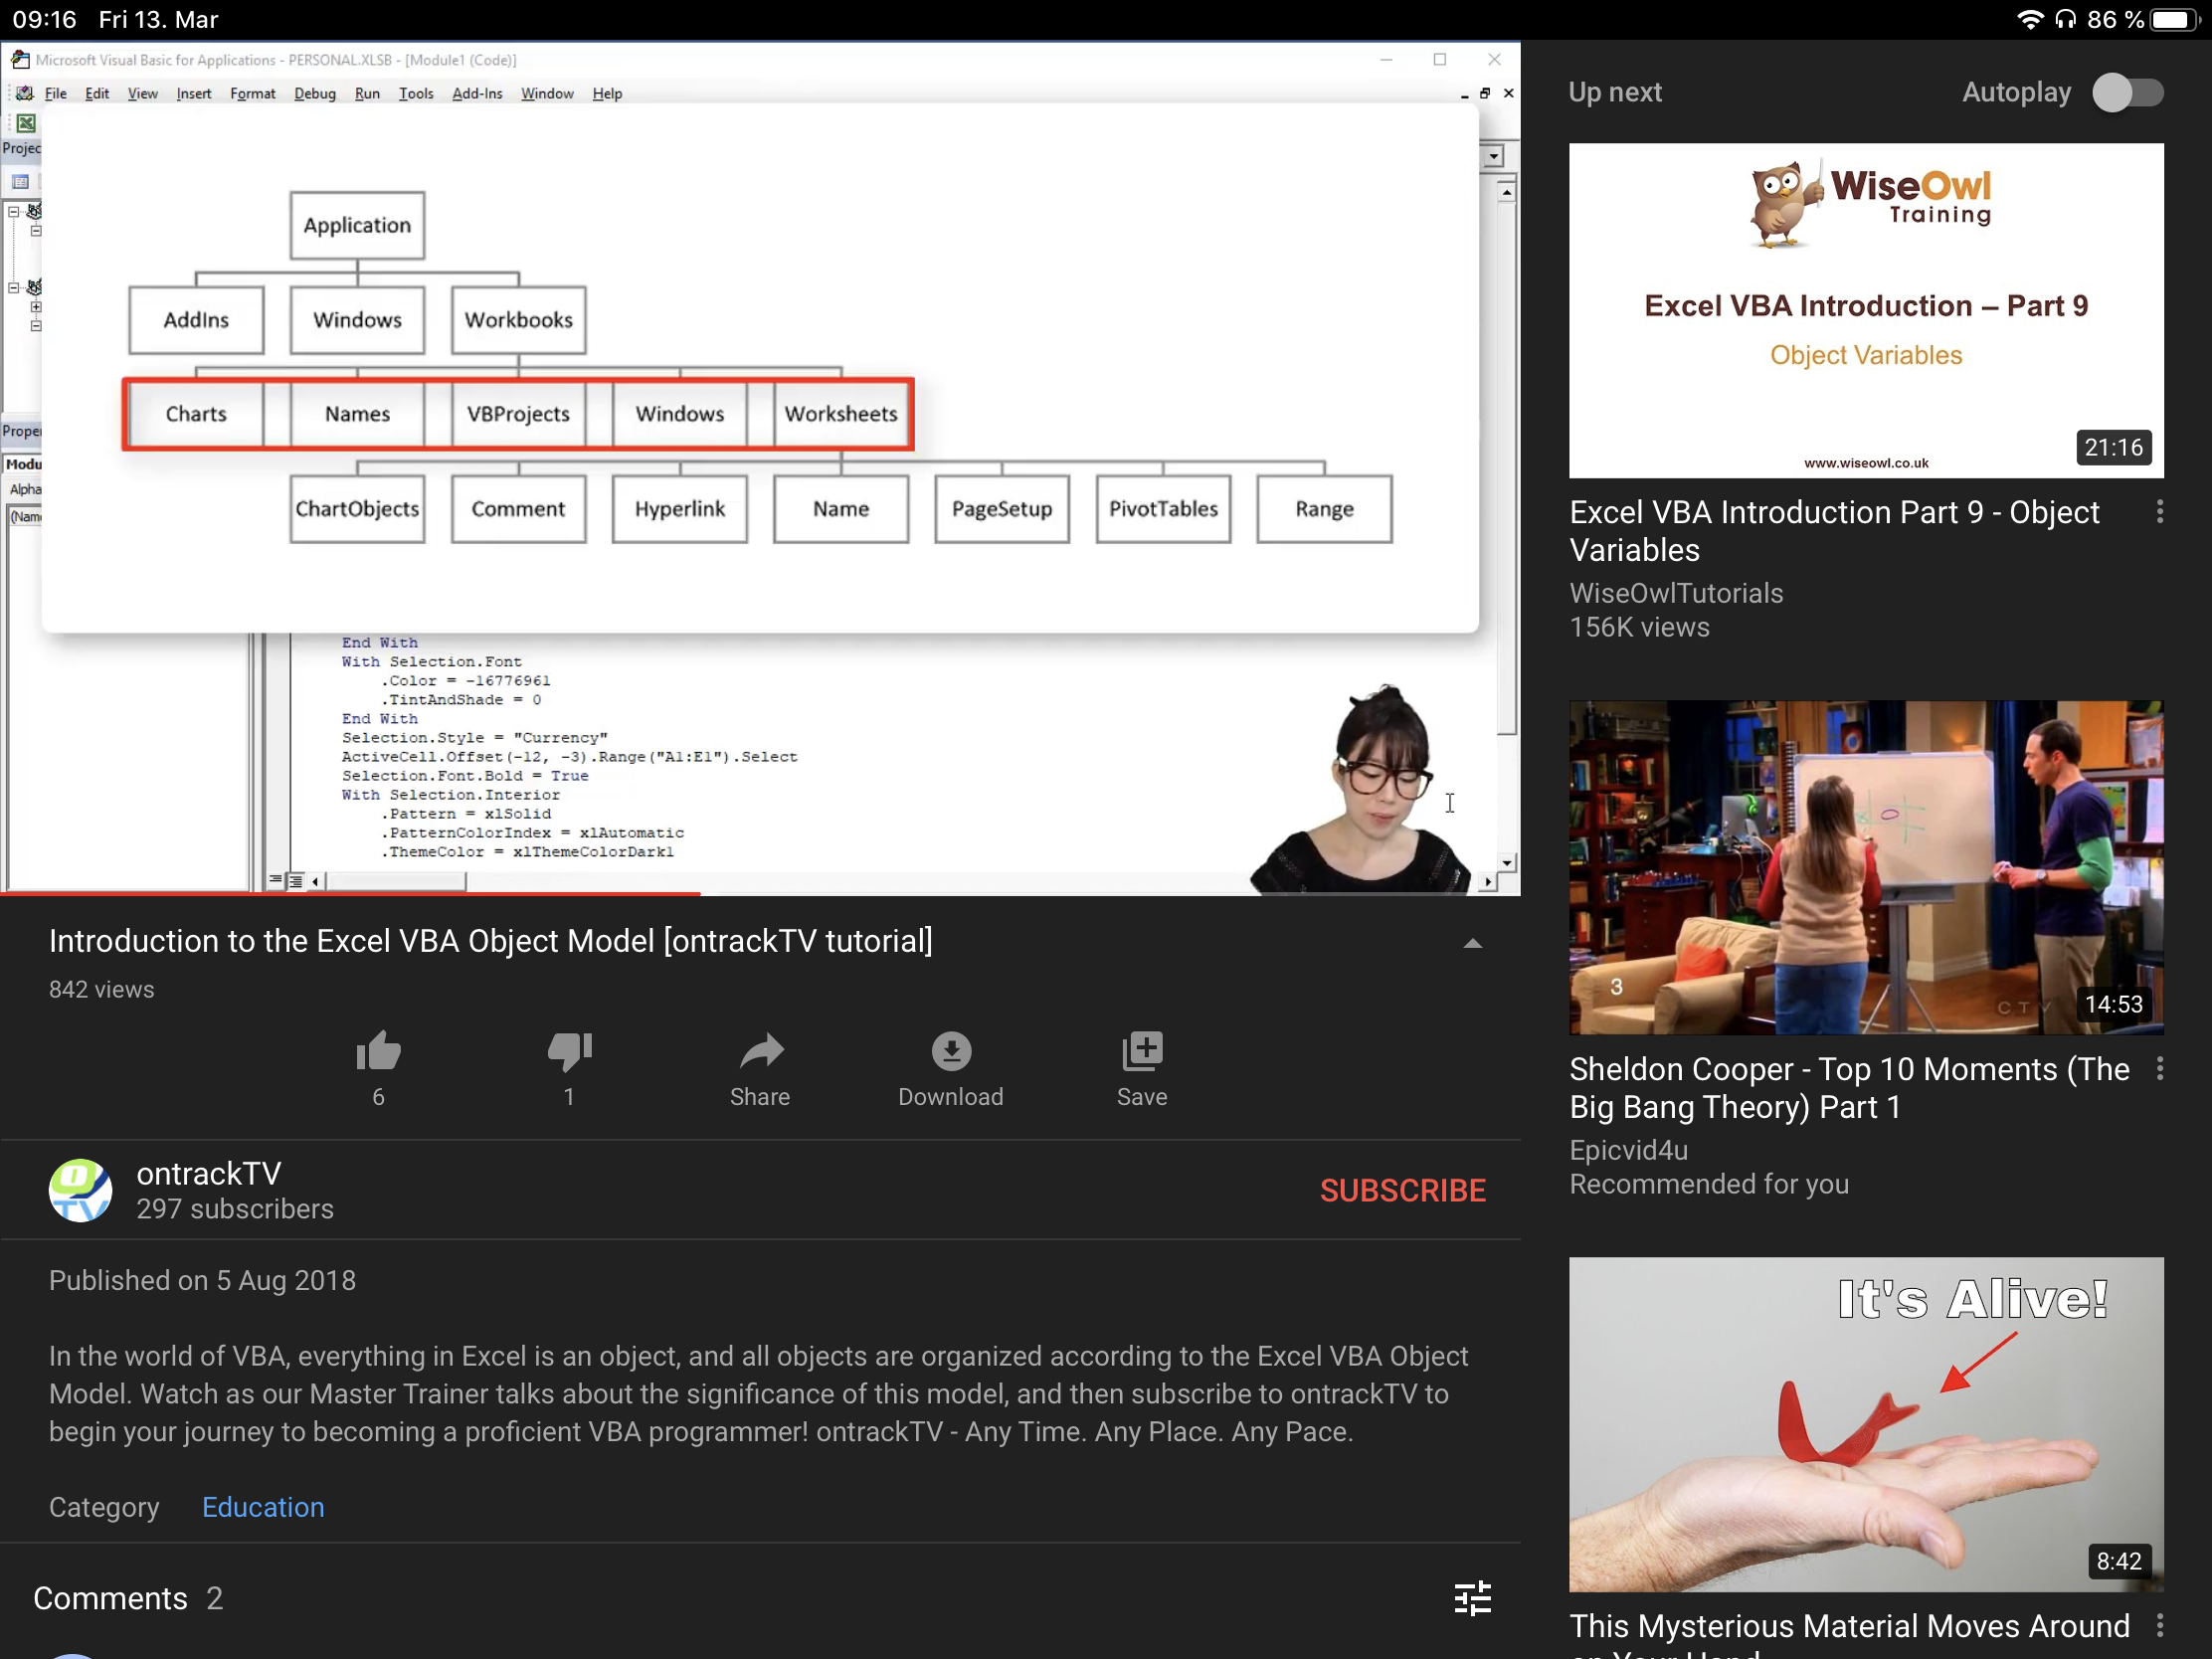
\includegraphics[scale = 0.3]{attachment/chapter_2/Scc020}
	\caption{}
	\label{fig:Scc020}
\end{figure} 
Auf der object model wird vermutlich im späteren Verlauf nochmal eingegangen. Aktuelle wird im Kurse weiter vorangeschritten, um vielleicht das fehlende Verständnis über das Model aufzuarbeiten. 
\subsubsection{VBA Editor}
Der Editor bietet über \textbf{F2} die Möglichkeit an, die Hilfefunktion abzurufen.
\begin{figure}[H]
	\centering
	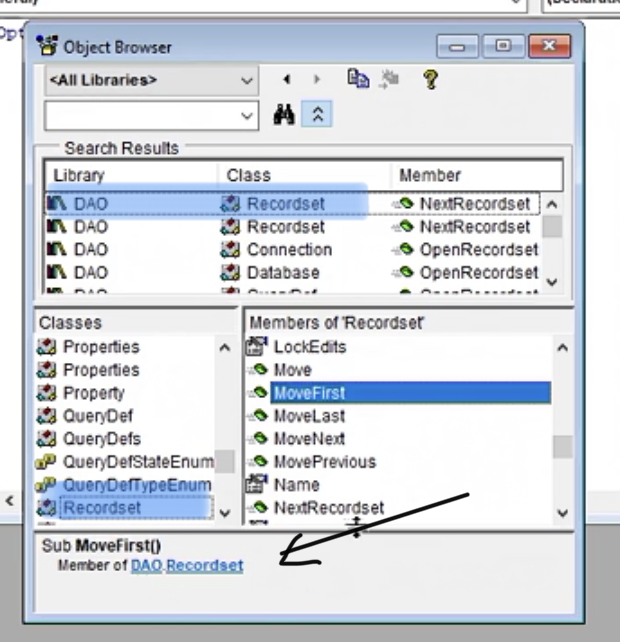
\includegraphics[scale = 0.3]{attachment/chapter_2/Scc021}
	\caption{}
	\label{fig:Scc021}
\end{figure} 
Eine der einfachsten \textit{Expressions} ist die Message Box. Die Funktion dazu lautet 

\begin{lstlisting}[style=VBA]
	Sub MessageBox ()
		MsgBox "Hello Paul."
	End Sub
\end{lstlisting}
\subsubsection{Processor: Subroutine and function}
In diesem Kontext ist es sinnvoll darüber zu sprechen, dass \gls{VBA} zwischen Objekt-Module und Module unterscheidet.
Subroutinen können Werte übertragen bekommen. \\

\begin{lstlisting}[style=VBA]
	Sub DatabaseName ()
		Dim sDbName As String ' Variablennamen können mit einem Kleinbuchstaben geginnen.
		sDbName =  "Paul" 
	End Sub
	
	Sub ShowDatabaseName (sDbName As String)
		MsgBox sDbName
	End Sub
\end{lstlisting}

\subsubsection{Processor: Function}
Der Unterschied zur $Sub$ ist, dass eine $function$ einen Wert zurückgeben kann. Ein $Sub$ nicht.
The $return$ ist called by the function name. Das bedeutet am Ende der Prozedur wird ein eine Ausgabe definiert. Diese muss mit den Namen der Funktion betitelt werden.

\begin{lstlisting}[style=VBA]
	Function MultiplikationPy (dZahl As double)
		MultiplikationPy = dZahl*3.14
	End function
	
	Sub Show ()
' 		MsgBox MultiplikationPy(5); Dies wird nicht funktionieren, da die Funktion ein double Wert benötigt.
	Dim dZahl As double
	dZahl = 5
	
	MsgBox MulitplikationPy(dZahl)
	End Sub
	
\end{lstlisting}


\subsubsection{Set Statement} 
The $Set$ statement is like a pointe in $C++$. \gls{VBA} hat eine Objekt-Hierarchy aufgebaut. Dabei können innerhalb dieser Hierarchy Objekte angesteuert werden - es wird auf sie verweisen. Mit $Set$ kann daraufhin innerhalb dieser Struktur Verweise geschaffen werden. Diese werden dann genutzt um Methoden abzurufen, auf weitere Objekte zu verweisen oder Werte auszulesen. Damit ist $Set$ zu unterscheiden von dem einfachen Datentypen, wie \textit{string, boole}. Die Verweise können zum einen mit einen einfachen \textit{Object} Typ deklariert werden, zum anderen können aber auch spezifischer Typen angegeben werden. 

\begin{lstlisting}[style=VBA]
	Dim wbObjekt As Workbooks ' Variable wird initialisiert
	Set Application.Workbooks("Name.xlxm") 
\end{lstlisting} 
Wir eine neue Instant eine Objektes erzeug, wird $New$ verwendet.
Bei der Deklarierung, $Set$, wird noch kein Objekt erzeugt, erst mit $Set$
\begin{lstlisting}[style=VBA]
	Dim myChildForms(1 to 4) As Form1 
	Set myChildForms(1) = New Form1 
	Set myChildForms(2) = New Form1 
	Set myChildForms(3) = New Form1 
	Set myChildForms(4) = New Form1
\end{lstlisting} 
 Es können natürlich mehrer Referenzen zu einem Objekt geschaffen werden. 

\begin{lstlisting}[style=VBA]
	Dim wbObjekt As Workbooks 
	Set wb = Application.Workbooks("Name.xlxm")
	Set wb2 = Application.Workboos("Name.xlxm")
\end{lstlisting} 

\subsubsection{First Code-Marco}
Wir ein Command Button erstellt, kann dieser über die Funktion \textit{Event Builder} angesteuert werden.

\begin{figure}[H]
	\centering
	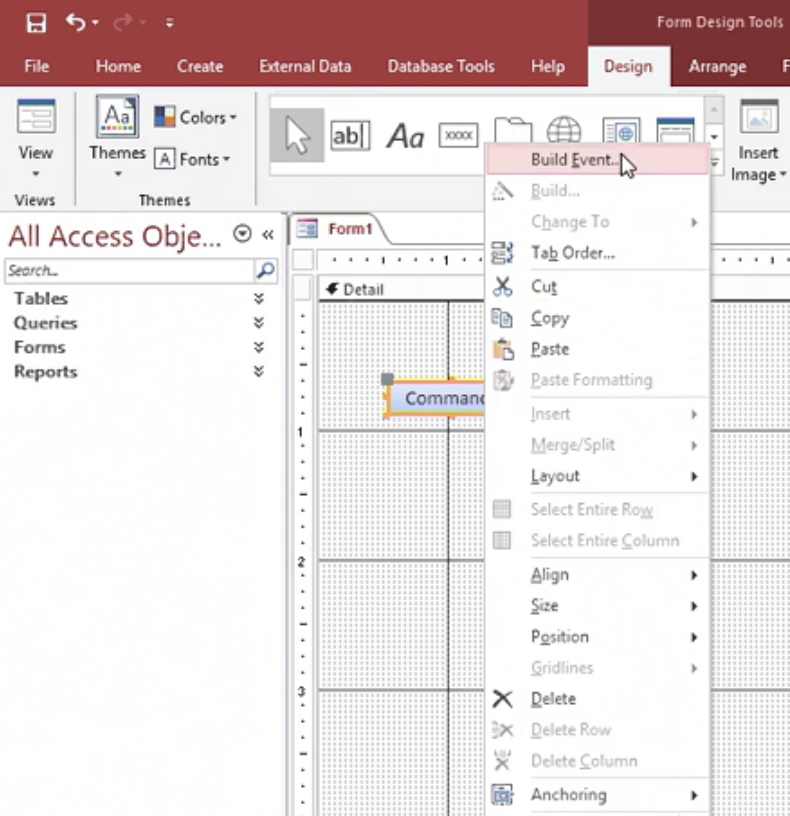
\includegraphics[scale = 0.3]{attachment/chapter_2/Scc022}
	\caption{}
	\label{fig:Scc022}
\end{figure} 

\begin{figure}[H]
	\centering
	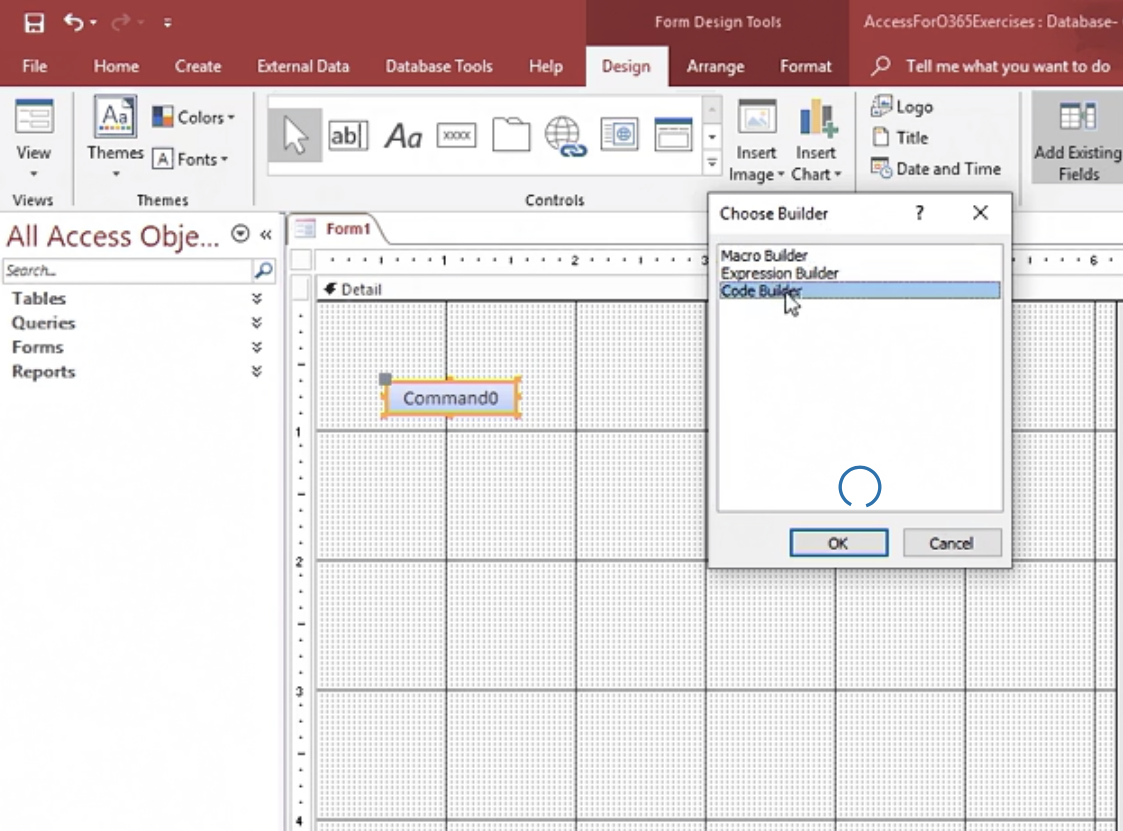
\includegraphics[scale = 0.3]{attachment/chapter_2/Scc023}
	\caption{}
	\label{fig:Scc023}
\end{figure} 

Es wird ein Makro (Code) erstellt. 
\begin{figure}[H]
	\centering
	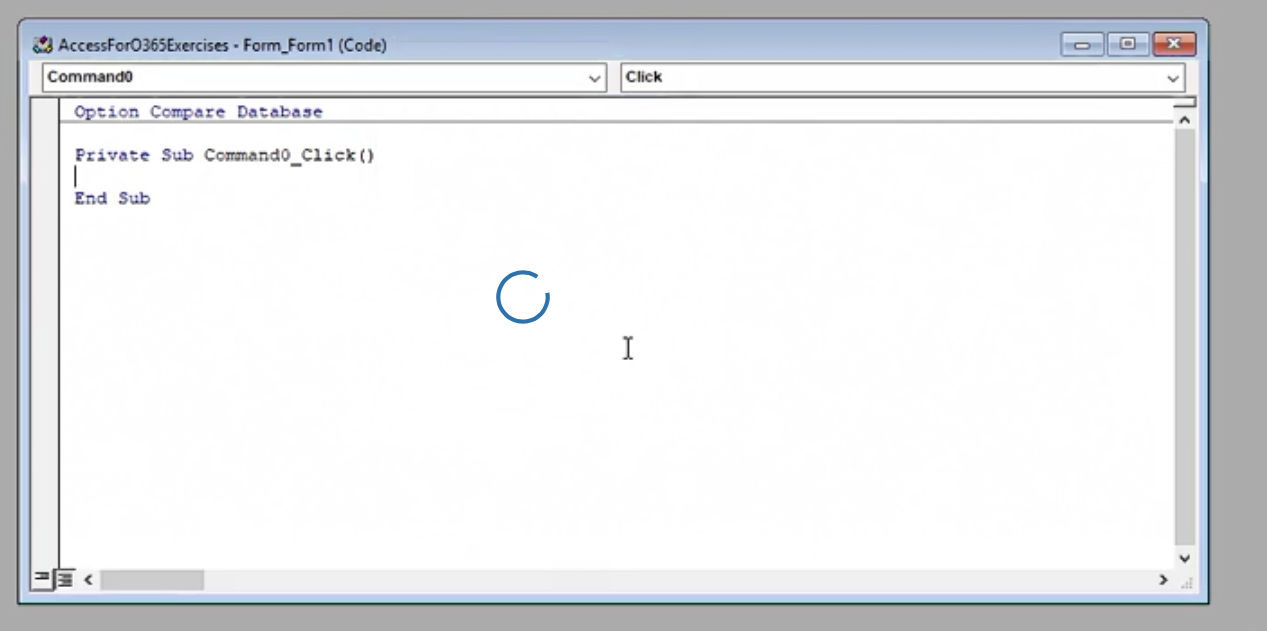
\includegraphics[scale = 0.3]{attachment/chapter_2/Scc024}
	\caption{}
	\label{fig:Scc024}
\end{figure} 
Die Option \textit{Option Compare Database} hat die Funktion, dass die folgenden Prozeduren auf Groß- und Kleinschreibung bei einem String-Vergleich nicht berücksichtig wird. Ebenso wird das Module unter dem Formblatt abgespeichert.

\begin{figure}[H]
	\centering
	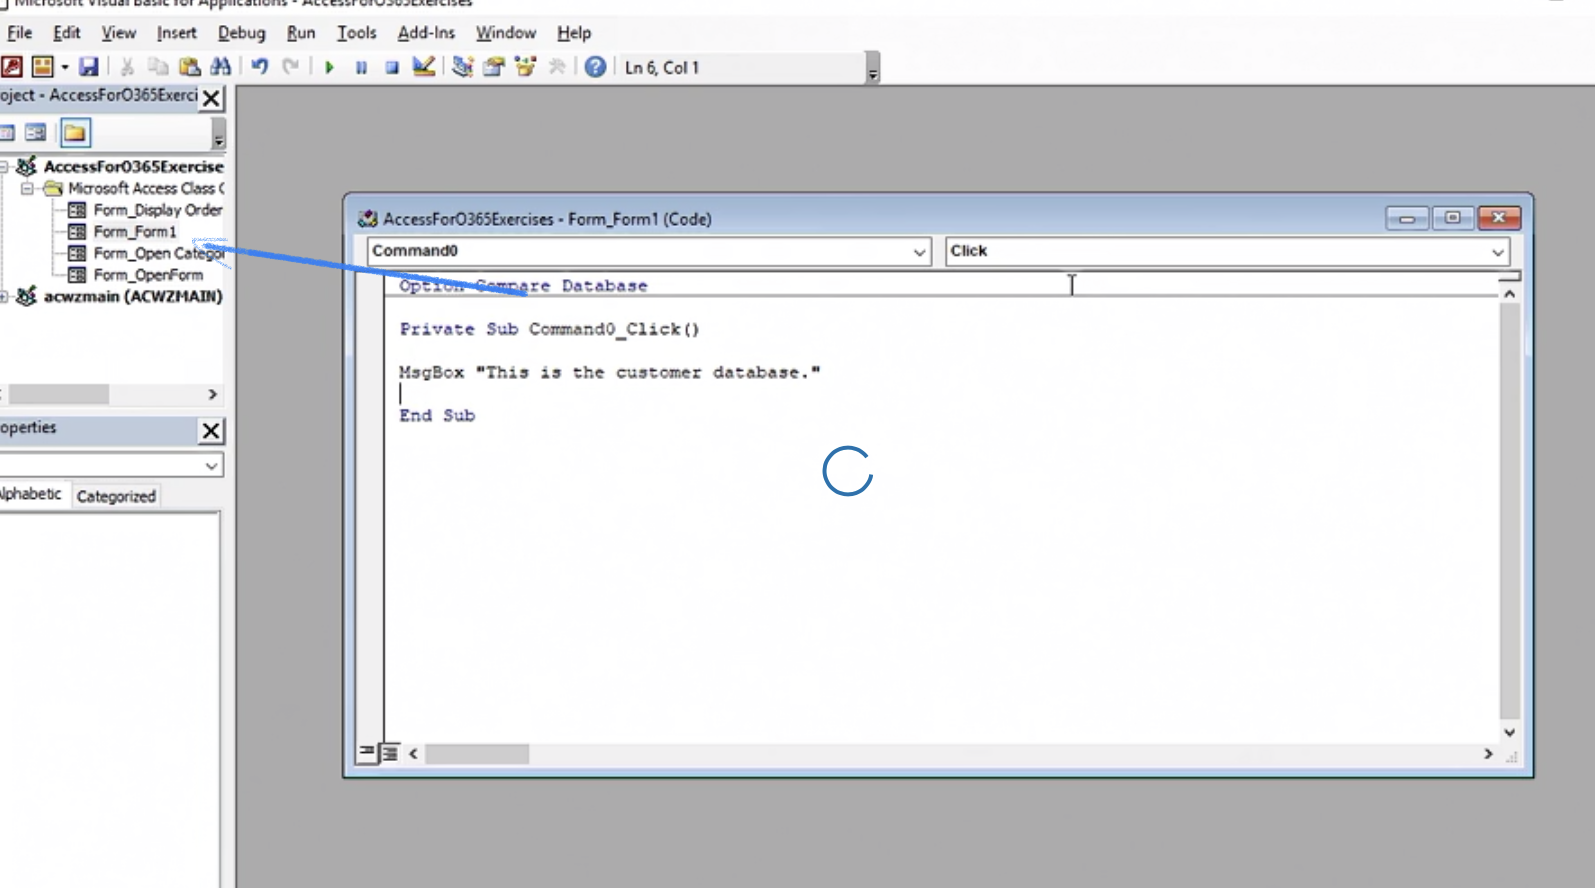
\includegraphics[scale = 0.3]{attachment/chapter_2/Scc025}
	\caption{}
	\label{fig:Scc025}
\end{figure} 

So weit ich es verstanden habe, ist ein Form Objekt ein angesteuertes Object welches sich in Forms Objekt befindet. Methoden die für Form vorgesehen werden, können erst durch ein genaues ansteuerten eines einzelnen Form ausgeführt werden. 
\begin{lstlisting}[style=VBA]
	Sub AddressObject()
		Dim myForm As Form
		Set myForm = Forms("Product") ' Use of a different object
		MsgBox myForm.Name
		Set myForm = Nothing ' Releases the connection
	End Sub
\end{lstlisting}


\subsection{Variables, Constants, Calculation}
Die Option \textit{Option Explicit} zwingt, dass alle Variablen deklariert werden müssen.
Variablen die außerhalb von Prozeduren stehen, werden als globale Variablen definiert und sind für das gesamte Modul verfügbar. 
\begin{lstlisting}[style=VBA]

	Dim iNumber As Integer = 20 ' Global
	Const iNumber2 As Integer = 30 ' Global und behält den konstanten Wert
	Static iNumber3 As Integer = 40 ' Global und behält den Wert über mehrere Ausführungen
	Sub Main()
		'
	End Sub
\end{lstlisting} 
\subsection{Add Logic to your VBA Code}
\subsubsection{Iterator-Prozeduren} 
\begin{itemize} 
\item For ... to ... Next: Integer Loop-Schleife 
\item For each ... in ... Next: Iteriert durch eine Array durch. 
\begin{lstlisting}[style=VBA]
Sub ForEach()
	Dim varItem As Variant
	Dim varArray As Variant
	
	varArray = Array("Eins", "Zwei", "Drei")
	
	For each varItem in varArray
	MsgBox (varItem)
	Next	

End Sub
\end{lstlisting}   
Für das Form-Collection kann ebenfalls so angesteuert werden.
\begin{lstlisting}[style=VBA]
Sub ForEachForm()
	Dim myF As Form
	
	For Each myF in Forms
	MsgBox (myF.Name)
	Next

End Sub
\end{lstlisting} 
\item Do until ... Loop: 
\item Do while ... Loop: \\ Es gibt verschiedene Syntaxen/ Methoden um auf Spalten in einem Recordset zu verweisen.
\begin{itemize}
\item Itemmethode: myR!["Nachname"]
\item Fields: myR.Fields("Nachname")
\end{itemize}
Der Verweis start immer am Anfang eines Tabelle. Der Loop muss jedoch separat gesteuert werden. In M wird die über die Funktion gesteuert und per each wird jede Zeile umgewandelt. Wir die \textit{Recordset}.AddNew() Methode gestartet, zeigt der Zeiger am Ende der Tabelle.
\begin{lstlisting}[style=VBA]
Sub Ausgabe_Print()	
	Dim recTest As Recordset
	Dim i As Long 
	Set recTest = Currentdb.OpenRecordset("Tabelle")
	
	Do while i < recTest.RecordCount ' Oder recTest.EOF (Endoffile)
	Debug.Print recTest.Fields("Nachname") ' Alle Daten in der Spalte Nachname werden ausgegeben.
	i = i + 1
	recTest.Move
	End Sub
\end{lstlisting} 
 \item If else; elseif
 \item Case Statment
\end{itemize}
\subsection{Debug Code}
\begin{itemize}
\item Siehe unter Fehlerbehandlung/VBA-Tutorial. 
\item Breakpoint. Klickt man am linken Rand im Editor wird ein roter Punkt gesetzt. Dieser stellt ein Breakpoint da. 
\begin{figure}[H]
	\centering
	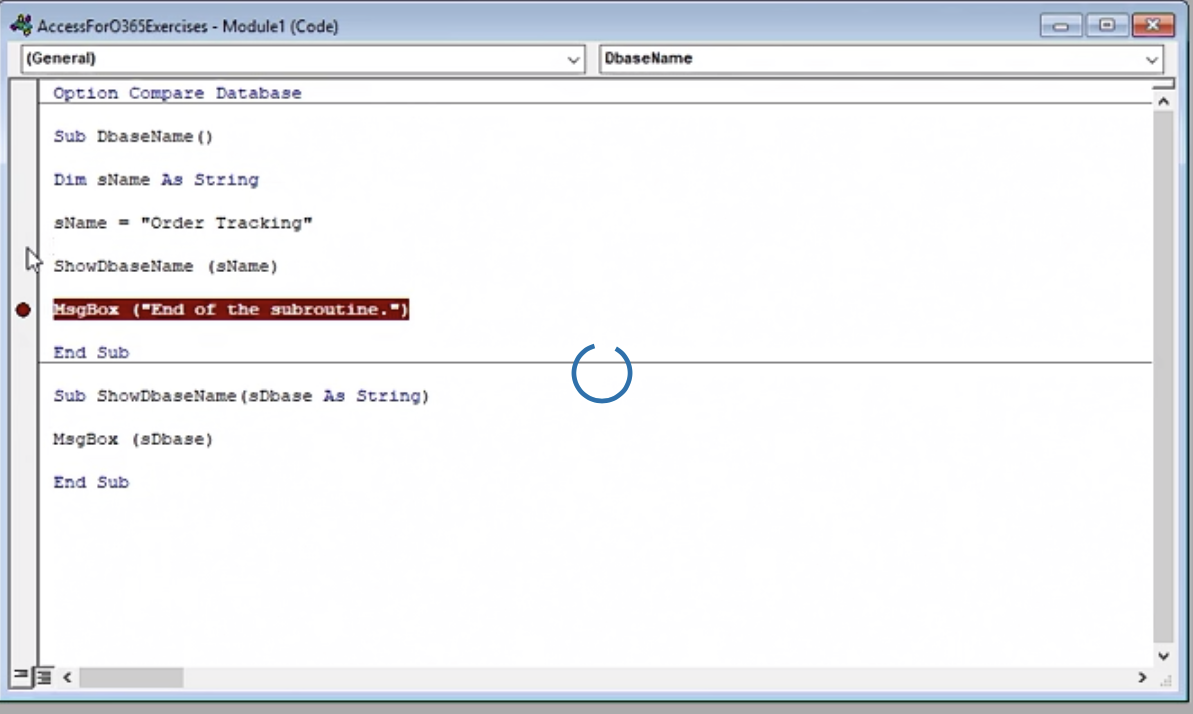
\includegraphics[scale = 0.3]{attachment/chapter_2/Scc061}
	\caption{}
	\label{fig:Scc061}
\end{figure} 
\item Add Watch
\end{itemize}

\subsection{Manipulate Database Object using DoCmd Object}
\subsubsection{Open Objects} 
\begin{description}
\item[DoCmd OpenForm] Diese Funktion bietet viele Option die Form in spezieller Weise zu öffnen: DoCmd.OpenForm
\item[DoCmd OpenRecord] Ein Record wird gleich an den Drucker gesendet. Um nur ein Report sich anzeigen zulassen, muss die Funktion abgeändert werden.
\item[DoCmd OpenTable] Mit DoCmd.OpenTable "Name" wird die dazugehörige Tabelle geöffnet.
\end{description}  
 Die verschiedenen Ansichtsmodi helfen das Objekt im richtigen Modus zu öffnen.

\subsubsection{Close Objects}
Um ein Objekt zu schließen, kann 
\begin{lstlisting}[style=VBA]
	DoCmd.Close acForm "Name"
\end{lstlisting}  
Unter \bl{ac} wird das Objekt spezifiziert und über den Namen direkt angesteuert.

\subsubsection{RunCommand Export}
Unter DoCmd.RundCommand befinden sich die Menüoptionen. Diese können über diese Methode aufrufen. Am Beispiel Daten zu exportieren, wird der Befehl acCmdExportExcel ausgewählt.

\begin{lstlisting}[style=VBA]
	DoCmd.RunCommand (acCmdExportExcel)
\end{lstlisting}  
\subsection{Read and manipulate Table Data}
\subsubsection{Add New}
Es ist wichtig, dass nach dem die Methode AddNew() ausgewählt und die Eingaben getätigt wurden, die UpDate() Methode aufgerufen wird, um die Eingaben zu speichern.
\subsubsection{Edit}
Die Methode Edit() erlaubt einen spezifischen Datensatz zu bearbeiten. Es ist dabei wichtig vor her die entsprechende Zeile zu finden. Eine Methode, die spezifische Datensätze sucht, ist FindFirst(). 
Ebenfalls wird UpDate() benötigt.
\subsubsection{Data Perservation} 
Um den Nutzer einzubinden, ob die geänderten Einträge auch wirklich verwendet werden sollen, wird gern die Transaktions-Mehtoden verwendet.
\begin{itemize}
\item BeginTrans()
\item CommitTrans()
\item RollbackTrans()
\end{itemize}
Diese Methoden können für verschiedenen Objekte angewandt werden. Es bietet sich an, .Workspace(0) zu verwenden. Ebenso, kann der Nutzer aufmerksam gemacht werden, ob er die Änderungen anwenden möchte.
\begin{lstlisting}[style=VBA]
Sub Preserv()
	Dim worVar As Workspace
	Dim recVar As Recordset
	Set worVar = DAO.DBEngine.Workspace(0)
	Set recVar = DAO.Currentdb.OpenRecordset("Name")
	
	worVar.BeginTrans()
	
	Do Until recVar.EOF
	
	'Stuff
	
	Loop
	
	If MsgBox ("Do you want the Change?", vbQuestion + vbYesNo) = ybYes Then
		worVar.CommitTrans()
	Else
		worVar.RollbackTrans()	
	
End Preserv
\end{lstlisting} 
\subsubsection{TableDef}
Diese Objekt ist unter Currentdb zufinden. Mit Hilfe dieses Objektes können unteranderem Eigenschaften eines Feldes abgerufen werden.

\subsection{Manipulate a Database using the Application Object}
\subsubsection{Function to Summarize}
\begin{itemize}
\item DAvg() - Nimmt den Average über eine Spalte hinweg: DAvg("Quanität") 
\item DMax(), DCount(), DMin(), etc.
\item DFirst(), DLast() - Bei diesen beiden Funktionen wird die Tabelle als String verwendet: DFrist("Spaltenname", "Tabellennamen"
\end{itemize}   
\subsubsection{DLookup()}
Die DLookUp() Funktion gibt die Werte aus einer anderen Tabelle oder Querie wieder.
\begin{lstlisting}[style=VBA]
DLookUp(
	"[Spalte_Wiedergabe_Sekundär]", //- Der Wert der gesucht wird, aus einer meist anderen Tabelle/ Query.
	"Tabelle_Sekundär", //- Andere Tabelle/ Query
	"[Spalte_Suche_Sekundär] =" & [Spalte_Suche_Primär]) //- Vergleiche Spalten aus der zu suchenden Tabelle und aus der erstellten Tabelle. 
\end{lstlisting} 

\subsection{Control Forms and Reports}
\subsubsection{Sinnvolle Einschränkugen}
\begin{itemize}
	\item Damit Nutzer nicht Daten einfach ändern, löschen oder hinzufügen, kann dies direkt über Eigenschaften der Forms gesteuert werden. 
	Gesteuert werden die Eigenschaften am Besten, wenn das Objekt geladen wird. 
	\begin{lstlisting}[style=VBA]
	Sub Form_Load()
	Me.AllowAdditions = False
	Me.AllowEdits = False
	Me.AllowDeletions = False
	End Sub
	\end{lstlisting}
	\item Ebenso kann die Filterfunktion deaktiviert werden. Dies können auch in Formular angewandt werden.
	\begin{figure}[H]
		\centering
		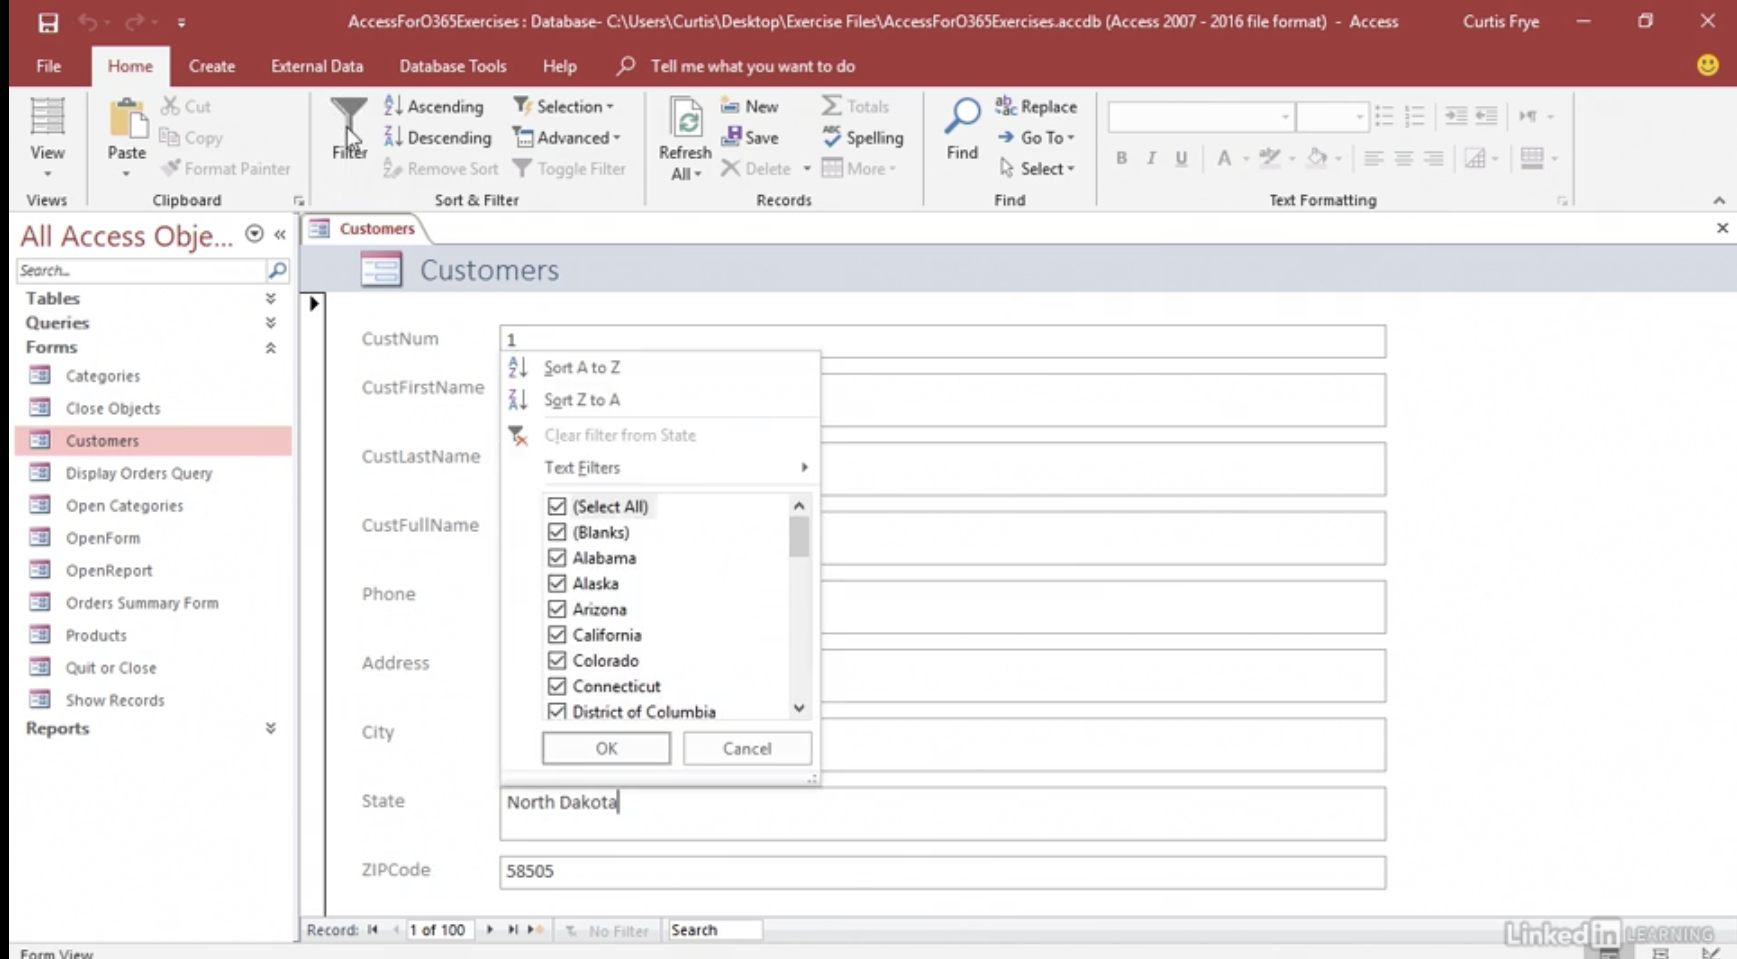
\includegraphics[scale = 0.3]{attachment/chapter_2/Scc062}
		\caption{}
		\label{fig:Scc062}
	\end{figure} 
	Um diese Funktion nicht mehr zu erlauben.
	\begin{lstlisting}[style=VBA]
	Sub Form_Load()
	Me.AllowFilter = False
	End Sub
	\end{lstlisting} 
	Wir das Formular neu geladen, so ist die Filter-Funktion ausgeblendet.
	\begin{figure}[H]
		\centering
		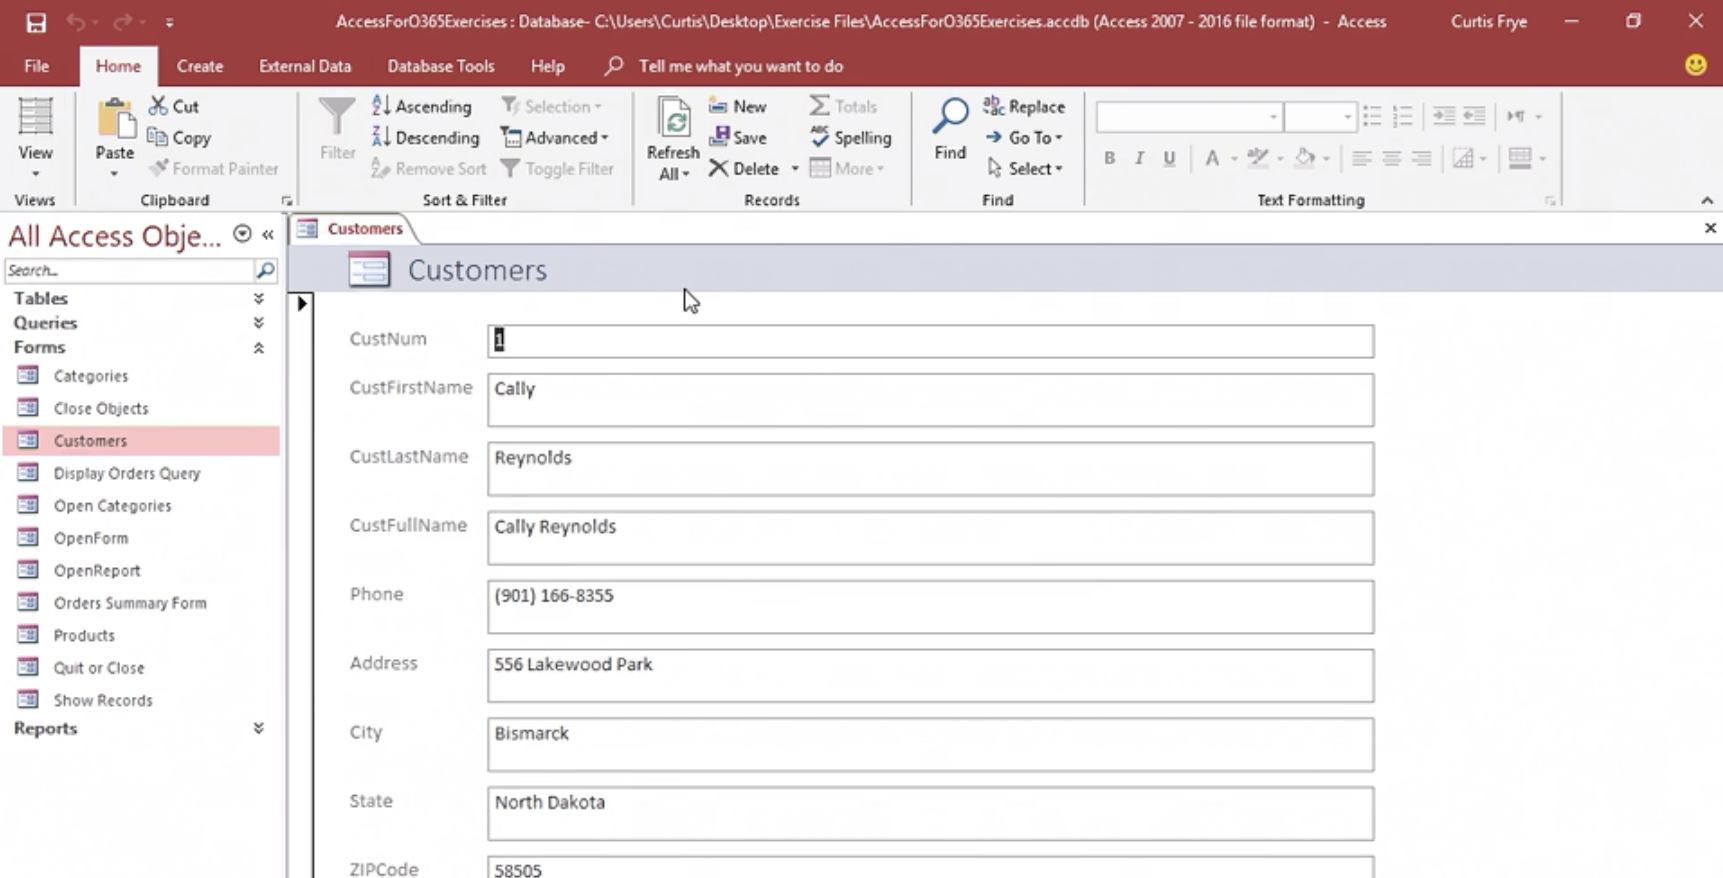
\includegraphics[scale = 0.3]{attachment/chapter_2/Scc063}
		\caption{}
		\label{fig:Scc063}
	\end{figure}
\end{itemize}


\subsubsection{Verfeinerung}
\begin{description}
	\item[Dynamische Beschriftung] Der Hintergrund, sowie die Überschrift eines Formulars und Report können direkt über das \bl{Me.} Objekt angesteuert werden. 
	\item[Aktualisierung des Formulars] Wird direkt ein Wert in der Tabelle hinterlegt, so ändert dies nicht automatisch die abgefragten Daten im dazugehörigen Formular. Mit \bl{Me.Requery} wird unter \bl{Form}$\_$\bl{Activate()} das Formular eine neue Abfrage starten, sobald es das aktive Fenster wird.
	\item 
\end{description}